\chapter{Modélisation d'un drone convertible : DarkO}
\minitoc
\label{chap:model}

\section{Modèle du drone DarkO}
\label{sec:model}
DarkO, drone conçu et développé à l'École Nationale de l'Aviation Civile (ENAC) de Toulouse (France), est un exemple de drone convertible avec une architecture dite \textit{tailsitter}.
DarkO est assemblé à partir de plusieurs pièces d'Onyx imprimées en 3D (un matériau très robuste composé de fibres de carbone omnidirectionnelles). Toutes les pièces sont emboîtées sur un seul axe, de sorte que le drone puisse facilement être démonté pour remplacer des pièces ou accéder à l'électronique embarquée. 

\nomenclature[]{\(ENAC\)}{École Nationale de l'Aviation Civile}

L'autopilote embarqué est une carte Apogee~\footnote{\url{https://wiki.paparazziuav.org/wiki/Apogee/v1.00}} fabriquée à l'ENAC (voir Fig. \ref{fig:apogee}). 


\begin{figure}[ht!]
    \centering
        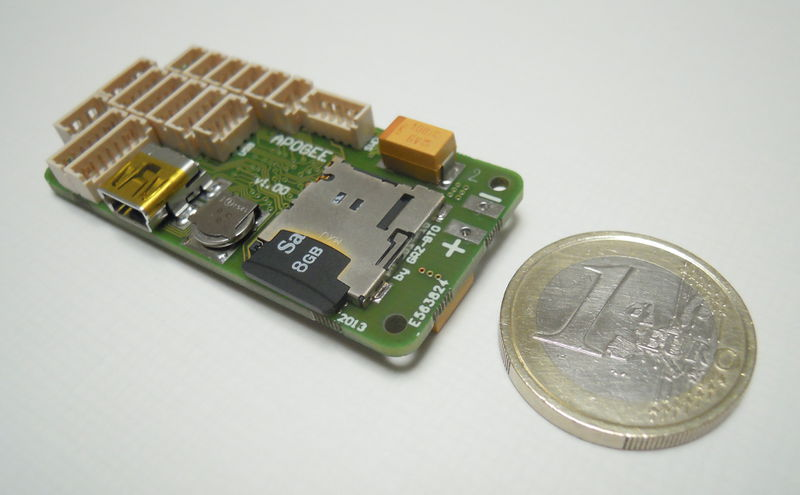
\includegraphics[width=0.5\columnwidth]{figures/800px-Apogee_v100_top_1E.jpeg}
        \caption{Vue de dessus d'un autopilote Apogee v1.00.}
        \label{fig:apogee}
\end{figure}

L'autopilote offre la possibilité d'enregistrer les données de bord sur une carte mémoire SD, à la fréquence de contrôle de 500 Hz, ce qui permet un post-traitement efficace des données acquises. Le protocole de communication utilisé entre l'autopilote et les contrôleurs électroniques de vitesse (ESC) est le Dshot 600. Les ESC sont des AIKON AK32 35A avec un \textit{firmware} AM32. La communication sol-bord est réalisée via un canal bidirectionnel basé sur des modules XBee-PRO S1.

\nomenclature[]{\(ESC\)}{Contrôleurs électroniques de vitesse (\textit{Electronic Speed Controller})}

\begin{figure}[ht!]
    \centering
    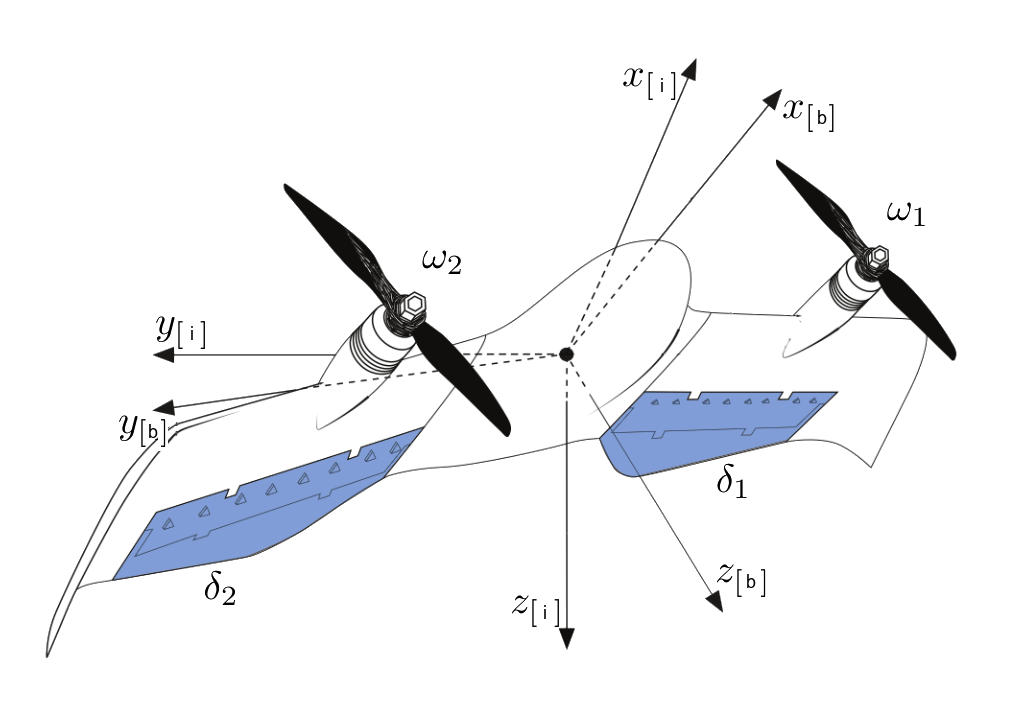
\includegraphics[width=0.8\columnwidth]{figures/darko.png}
    \caption{Repère de référence de DarkO avec une représentation schématique des actionneurs.}
    \label{fig:darko2}
\end{figure}
Les actionneurs de DarkO sont deux catégories. La première est liée à la propulsion et est constituée de deux hélices (T-Motor T5147) placées symétriquement à l'avant de l'aile (illustrées en \textbf{noir} dans la Fig. \ref{fig:darko2}) et alimentées par deux moteurs électriques (T-Motor F30 2300kv) générant une traction selon l'axe $x_{b}$. La seconde catégorie est relative aux actionneurs aérodynamiques. Ainsi, le drone possède deux élevons, placés à l'arrière de l'aile (illustrés en \textcolor{cyan}{bleu} dans la Fig. \ref{fig:darko2}), agissant en tant que surface de contrôle. Les élevons génèrent des forces et des moments en modifiant leur incidence relativement au flux d'air dans lequel ils sont placés.  Ce flux d'air peut être dû au vent relatif (lié à la vitesse du drone), au vent extérieur, mais aussi au souffle des hélices. Les élevons sont commandés par deux servomoteurs MKS DS65K qui apporte une grande rapidité lors des déplacements avec une grande robustesse et une faible masse.

La figure \ref{fig:darko2} montre le modèle de DarkO, ainsi qu'un repère de référence inertiel \textit{North, east, down} (NED) \nomenclature[]{\(NED\)}{Nord Est Bas (\textit{North, East, Down})} (ou repère terrestre) ``$\text{i}$'' lié à la surface de la Terre, et un repère corps `$\text{b}$'' attaché au drone, avec $x_{\text{b}}$ correspondant à l'axe de roulis (l'axe des hélices dans le plan $z_{\text{b}} = 0$), $y_{\text{b}}$ l'axe de tangage (la direction des ailes), $z_{\text{b}}$ l'axe de lacet. En utilisant la même notation que dans \cite{lustosaHal-03035938}, le couple hélice/élevon gauche et droit est désigné par les indices $i=1$ (gauche) et $i=2$ (droite). La convention de signe sera définie comme positive pour les positions des élevons $\delta_{1}$, $\delta_{2}$ lorsqu'ils créent un moment à cabrer avec les hélices tournant dans des directions opposées avec des vitesses angulaires $\omega_{1} > 0$ et $\omega_{2} < 0$, respectivement.

\begin{table}[h]
    \centering
      \begin{tabular}{|l|c|c|}
        \hline
        \multicolumn{1}{|c|}{Paramètres et coefficients} & Valeurs & Unités \\
        \hline
        $m$ (Masse du drone)  & 0.519 & \SI{}{\kilogram} \\
        \hline
        $b$ (Envergure)  & 0.542 & \SI{}{\meter} \\
        \hline
        $c$ (Corde aérodynamique)  & 0.13 & \SI{}{\meter} \\
        \hline
        $\boldsymbol{B}=\diag(b,c,b)$ & $\!\!\diag(0.542, 0.13, 0.542)$ \!\! & \SI{}{\meter}\\
        \hline
        $S$ (Surface de l'aile) & 0.026936 & \SI{}{\square\meter}\\
        \hline
        $S_{\text{wet}}$ (Surface soufflée) & 0.0180 & \SI{}{\square\meter}\\
        \hline
        $S_{\text{p}}$ (Surface des hélices) & 0.0127 & \SI{}{\square\meter}\\
        \hline
        $\boldsymbol{J}=\diag(J_{x},J_{y},J_{z})$ & \!\! $\diag(0.0067,0.0012,0.0082)$\!\! & \SI{}{\kilogram\square\meter}\\
        \hline
        $k_{\text{f}}$ (Poussée des hélices) & 1.7800e-8 & \SI{}{\kilogram\meter}\\
        \hline
        $k_{\text{m}}$(Moment des hélices) & 2.1065e-10 & \SI{}{\kilogram\square\meter}\\
        \hline
        $p_{x}$ (Position en $x$ des hélices) & 0.065 & \SI{}{\meter}\\
        \hline
        $p_{y}$ (Position en $y$  des hélices) & 0.162 & \SI{}{\meter}\\
        \hline
        $a_{y}$ (Position en $y$ de la portance) & 0.1504 & \SI{}{\meter}\\
        \hline
        $\xi_{\text{f}}$ (Portance des élevons) & 0.2 & --\\
        \hline
        $\xi_{\text{m}}$ (Moment des élevons) & 1.4 & --\\
        \hline
        $\rho$ (Densité de l'air) & 1.225 & \SI{}{\kilogram\per\cubic\meter}\\
        \hline
        $C_{\text{d}}$ (Trainée) & 0.1644 & --\\
        \hline
        $C_{y}$ (Latéral) & 0 & --\\
        \hline
         $C_{\ell}$ (Portance) & 5.4001 & --\\
        \hline
        $\Delta_{\text{r}}$ (Centrage du drone) & -0.0145 & \SI{}{\meter}\\
        \hline
      \end{tabular}
      \caption{Paramètres numériques identifiés du modèle DarkO.}
      \label{tab:pars}
\end{table}

\subsection{Modèle non-linéaire complet}

En exploitant la modélisation présentée dans \cite{lustosaHal-03035938, olszaneckibarthHal-02542982} et récemment validée par \cite{MuraliMorenoLustosa2024}, un modèle précis de la dynamique de DarkO permet de relier la position  du centre de gravité $\boldsymbol{p} \in \real^3$, sa vitesse $\boldsymbol{v} = \dot{\boldsymbol{p}} \in \real^3$.

Son orientation est représentée par un quaternion unitaire $\boldsymbol{q} \in {\mathbb S}^3:=\{ \boldsymbol{q} \in \real^4 : |\boldsymbol{q}| = 1\}$ et $\boldsymbol{q} := \left[ \eta ~ \boldsymbol{\epsilon}^\top \right]^\top$. Nous avons donc $\eta$ qui représente la partie scalaire du quaternion et $\boldsymbol{\epsilon}$ qui représente la partie vectorielle du quaternion.

La vitesse angulaire $\boldsymbol{\omega}_{\text{b}}$, représentée dans le repère du corps telle que $\boldsymbol{\dot q} = \frac{1}{2}\boldsymbol{q} \otimes \smallmat{0 \\ \boldsymbol{\omega}_{{\text{b}}}}$, où $\otimes$ représente le produit hamiltonien (c'est à-dire le produit de quaternions) couramment utilisé dans le contexte des quaternions. 
Le produit hamiltonien est défini par :
\begin{align}
    \label{eq:produitquat}
    p \otimes q = \begin{bmatrix}
        \eta_{p} \eta_{q}- \boldsymbol{\epsilon}_{p} \cdot \boldsymbol{\epsilon}_{q}\\
        \eta_{p}\boldsymbol{\epsilon}_{q}+ \eta_{q}\boldsymbol{\epsilon}_{p} + \boldsymbol{\epsilon}_{p} \times \boldsymbol{\epsilon}_{q}
    \end{bmatrix}.
\end{align}

En choisissant l'état global comme $\boldsymbol{x}:=(\boldsymbol{p},~ \boldsymbol{v},~ \boldsymbol{q},~ \boldsymbol{\omega}_{\text{b}})$, le modèle mathématique, dérivé dans \cite{lustosaHal-03035938}, dépend d'un ensemble de paramètres énumérés dans la Table~\ref{tab:pars}. Les valeurs numériques sont obtenues à partir d'une identification du système \cite{sansouStage}, la démarche est expliquée section \ref{sec:identification}.

Le modèle dynamique peut être écrit comme ci-dessous :

\begin{subequations}\label{eq:dyna_orig}
    \begin{empheq}[left=\empheqlbrace]{alignat=2}
           \boldsymbol{\dot p} & &= & \boldsymbol{v} \label{eq:dyna_orig_a}\\
          \label{eq:dyna_orig_b}
          m\boldsymbol{\dot v} &&=& - m\boldsymbol{g} +  \boldsymbol{R}(\boldsymbol{q})\boldsymbol{F}_{\text{b}},\\
          \boldsymbol{\dot q} &&=& \frac{1}{2}\boldsymbol{q} \otimes \boldsymbol{\omega_{b}} \label{eq:dyna_orig_c}\\
          \label{eq:dyna_orig_d}
          \boldsymbol{J} \boldsymbol{\dot \omega_{\text{b}}} &&= &  - \skewsym{\boldsymbol{\omega}_{\text{b}}}\boldsymbol{J}\boldsymbol{\omega}_{\text{b}} + \boldsymbol{M}_{\text{b}},
    \end{empheq}
  \end{subequations}
  où $\boldsymbol{g}:=\smallmat{0 & 0& 9.81}^\top$ désigne le vecteur de gravité, $m\in \real$ est la masse, $\boldsymbol{J}\in \real^{3\times 3}$ est le moment d'inertie diagonal (voir Table~\ref{tab:pars}), la matrice de rotation correspondant au quaternion $q$ est $\boldsymbol{R}(\boldsymbol{q}) \in SO(3): = \{\boldsymbol{R}\in \real^{3\times 3}: \; \boldsymbol{R}^\top \boldsymbol{R} = \mathbb{I}_{3} \text{ et}\det (\boldsymbol{R})=1\}$ est défini comme (voir \cite{hamel_minhduc})
\begin{align}
    \label{eq:matrix_rot}
    \boldsymbol{R}(\boldsymbol{q}) := \mathbb{I}_{3} +2\eta \skewsym{\boldsymbol{\epsilon}} + 2\skewsym{\boldsymbol{\epsilon}}^{2}.
\end{align}


D'après \cite{lustosaHal-03035938}, le vecteur de force $\boldsymbol{F}_{\text{b}}$ et le vecteur de moment $\boldsymbol{M}_{\text{b}}$ dans \eqref{eq:dyna_orig} dépendent  premièrement de l'état du système $\boldsymbol{x}$, puis de la perturbation $\boldsymbol{w} \in \real^3$, représentant la vitesse du vent dans le référentiel inertiel, et enfin de la commande des actionneurs (voir Figure~\ref{fig:darko2}), comprenant la vitesse de rotation des deux hélices $\omega_1, \omega_2 \in \real$ et la déflexion des élevons $\delta_1, \delta_2\in \real$.

Considérons premièrement l'effet des commandes des actionneurs. Chaque hélice génère une poussée $\boldsymbol{T}_i$ orientée dans la direction $x$ du repère corps et un moment $\boldsymbol{N}_i$ selon le même axe :
\begin{align}
\label{eq:thrust}
\boldsymbol{T}_{i} \!:=\! \begin{bmatrix} \tau_{i} \\ 0 \\ 0 \end{bmatrix} \!:=\!
\begin{bmatrix} k_{\text{f}}\omega_{i}^{2} \\ 0 \\ 0 \end{bmatrix}\! , \;
\boldsymbol{N}_{i} \!:=\! (-1)^{i}  \frac{k_{\text{m}} }{k_{\text{f}}}\boldsymbol{T}_{i}, \quad i=1,2 .
\end{align} 

La position de chaque élevon $\delta_i \in \real$ est assignée par un servomoteur qui impose un niveau d'efficacité (en termes de déviation du courant d'air) quantifié par deux matrices antisymétriques :
\begin{align}
\label{eq:elevons_efficiency}
    \boldsymbol{\Delta}^{\text{f}}_{i} \!:=\! \begin{bmatrix} 0 & 0 & \xi_{\text{f}}\delta_{i} \\ 0 & 0 & 0 \\ -\xi_{\text{f}}\delta_{i} & 0 & 0 \end{bmatrix}\! ,\;
    \boldsymbol{\Delta}^{\text{m}}_{i} \!:=\! \begin{bmatrix} 0 & 0 & \xi_{\text{m}}\delta_{i} \\ 0 & 0 & 0 \\ -\xi_{\text{m}}\delta_{i} & 0 & 0 \end{bmatrix} \!, \quad i=1,2.
\end{align}
 Les paramètres constants $k_{\text{f}}$, $k_{\text{m}}$, $\xi_{\text{f}}$, $\xi_{\text{m}}$ apparaissant dans \eqref{eq:thrust} et \eqref{eq:elevons_efficiency} sont listés dans la Table~\ref{tab:pars}.\\
Avec les quantités ci-dessus, nous pouvons réarranger la dynamique donnée dans  \cite[eqns (97),~(98)]{lustosaHal-03035938} (voir aussi \cite{sansouStage}) et exprimer $\boldsymbol{F}_{\text{b}}$ et $\boldsymbol{M}_{\text{b}}$ dans \eqref{eq:dyna_orig} comme :
%
\begin{align}
\nonumber
    \boldsymbol{F}_{\text{b}} :={}&  \boldsymbol{T}_{1} + \boldsymbol{T}_{2} + \frac{S_{\text{wet}}}{4S_{\text{p}}} \boldsymbol{\Phi}^{\text{(fv)}} \Big( (\boldsymbol{\Delta}^{\text{f}}_1 - \mathbb{I}_{3} ) \boldsymbol{T}_{1} + ( \boldsymbol{\Delta}^{\text{f}}_2 - \mathbb{I}_{3}) \boldsymbol{T}_{2}\Big) \\ 
    \nonumber
    &+ \frac{1}{4} \rho S  \boldsymbol{\Phi}^{\text{(fv)}} \Big(\boldsymbol{\Delta}^{\text{f}}_1+ \boldsymbol{\Delta}^{\text{f}}_2 - 2 \mathbb{I}_{3} \Big) \lVert \boldsymbol{v_{\text{b}}} \rVert \boldsymbol{v_{\text{b}}}\\
     \label{eq:Fbdarko}
    &+ \frac{1}{4} \rho S \boldsymbol{\Phi}^{\text{(mv)}} \Big(\boldsymbol{\Delta}^{\text{f}}_1 + \boldsymbol{\Delta}^{\text{f}}_2 - 2\mathbb{I}_{3}\Big) \boldsymbol{B} \lVert \boldsymbol{v_{\text{b}}} \rVert  \boldsymbol{\omega}_{\text{b}}, 
\end{align}

\begingroup
    \allowdisplaybreaks
    \begin{align} 
        \nonumber
    \boldsymbol{M}_{\text{b}} :&=\boldsymbol{N}_{1} + \boldsymbol{N}_{2} + \skewsym{\smallm{p_x\\ p_y\\ 0}} \boldsymbol{T}_{1} + \skewsym{\smallm{p_x\\ - p_y\\ 0}} \boldsymbol{T}_{2}\\
        \nonumber
    &- \frac{S_{\text{wet}}}{4S_{\text{p}}} \bigg( \boldsymbol{B} \boldsymbol{\Phi}^{\text{(mv)}} (\boldsymbol{\Delta}^{\text{m}}_1- \mathbb{I}_{3} ) + \skewsym{\smallm{0 \\ a_y \\ 0}} \boldsymbol{\Phi}^{\text{(fv)}} (\boldsymbol{\Delta}^{\text{m}}_1 +\mathbb{I}_{3} ) \bigg) \boldsymbol{T}_{1} \\
        \nonumber
    & - \frac{S_{\text{wet}}}{4S_{\text{p}}} \bigg( \boldsymbol{B} \boldsymbol{\Phi}^{\text{(mv)}} (\boldsymbol{\Delta}^{\text{m}}_2 - \mathbb{I}_{3} ) +  \skewsym{\smallm{0 \\ - a_y \\ 0}} \boldsymbol{\Phi}^{\text{(fv)}} (\boldsymbol{\Delta}^{\text{m}}_2 + \mathbb{I}_{3}) \bigg) \boldsymbol{T}_{2} \\
        \nonumber
    & + \frac{1}{4} \rho S  \bigg( \Big(\skewsym{\smallm{0 \\ a_y \\ 0}} \!\!\! \boldsymbol{\Phi}^{\text{(fv)}}  + \boldsymbol{B} \boldsymbol{\Phi}^{\text{(mv)}} \Big) \boldsymbol{\Delta}^{\text{m}}_1 \\
        \nonumber
    &  + \Big( \skewsym{\smallm{0 \\ - a_y \\ 0}} \!\!\! \boldsymbol{\Phi}^{\text{(fv)}} + \boldsymbol{B} \boldsymbol{\Phi}^{\text{(mv)}}  \Big) \boldsymbol{\Delta}^{\text{m}}_2 - 2 \boldsymbol{B} \boldsymbol{\Phi}^{\text{(mv)}}  \bigg) \lVert \boldsymbol{v_{\text{b}}} \rVert \boldsymbol{v_{\text{b}}} \\
        \nonumber
    & +\frac{1}{4} \rho S \bigg(\!\! \Big(\!\! \skewsym{\!\smallm{0 \\ a_y \\ 0}\!}\!\!\! \boldsymbol{\Phi}^{\text{(mv)}} \! + \! \boldsymbol{B} \boldsymbol{\Phi}^{\text{(m$\omega$)}} \Big) \boldsymbol{\Delta}^{\text{m}}_1 \\
        \label{eq:Mbdarko}
    & +  \Big(\!\! \skewsym{\!\smallm{0 \\ - a_y \\ 0}\!} \!\!\! \boldsymbol{\Phi}^{\text{(mv)}} \! + \! \boldsymbol{B} \boldsymbol{\Phi}^{\text{(m$\omega$)}}  \Big) \boldsymbol{\Delta}^{\text{m}}_2 - 2 \boldsymbol{B} \boldsymbol{\Phi}^{\text{(m$\omega$)}}\!  \bigg)\!  \boldsymbol{B}  \lVert \boldsymbol{v_{\text{b}}} \rVert  \boldsymbol{\omega}_{\text{b}} ,
    \end{align}
\endgroup

où $\boldsymbol{v}_{\text{b}} := \boldsymbol{R}^\top(\boldsymbol{q}) (\boldsymbol{v}-\boldsymbol{w})$ représente la vitesse de l'air vue par le drone et exprimée dans le repère du corps. 

Dans ce travail, la description de $\boldsymbol{F}_{\text{b}}$ et $\boldsymbol{M}_{\text{b}}$ est simplifiée par rapport à celle proposée dans la $\phi$-théorie \cite{lustosaHal-03035938}. En effet, la valeur de $\phi$ a été identifier nulle ce qui engendre $\eta = \sqrt{\lVert \boldsymbol{v_{\text{b}}} \rVert^{2} + \phi c^{2} \lVert \boldsymbol{\omega}_{\text{b}} \rVert^{2}} = \lVert \boldsymbol{v_{\text{b}}} \rVert$ dans  \cite[équation (17)]{lustosaHal-03035938}.

La matrice des coefficients aérodynamiques constants 
$\boldsymbol{\Phi}:= \begin{bmatrix} \boldsymbol{\Phi}^{\text{(fv)}} & {\boldsymbol{\Phi}^{\text{(mv)}}}^\top \\ \boldsymbol{\Phi}^{\text{(mv)}} & \boldsymbol{\Phi}^{\text{(m$\omega$)}} \end{bmatrix} \in \real^{6 \times 6}$, est définie dans \cite[eqs. (6)--(9)]{olszaneckibarthHal-02542982} comme $ \boldsymbol{\Phi}^{\text{(fv)}} \!:=\! \diag(C_{\text{d}},C_{y}, C_{\ell})$ et
\begin{align*}
&\left[ \begin{array}{c|c}
    \boldsymbol{\Phi}^{\text{(mv)}}  &  \boldsymbol{\Phi}^{\text{(m$\omega$)}} 
\end{array}\right] :=\\ 
&\left[ \begin{array}{ccc|ccc}
    0 & 0 & 0    &                                          0.1396 & 0 & 0.0573 \\
    0 & 0 & \!\!\!\!\! -\frac{\Delta_{\text{r}}}{c}C_{\ell} &    0 &  0.6358  & 0 \\
    0 & 0 & 0 &     0.0405 & 0 & 0.0019 
\end{array}\right].
\end{align*}


\subsection{Modèle non linéaire simplifié à basse vitesse}
\label{sec:model_NL_simp}

Dans la mesure où nous allons nous intéresser au maintien du drone en stationnaire, c'est-à-dire avec une vitesse du drone faible, nous pouvons simplifier la dynamique \eqref{eq:dyna_orig} en négligeant les effets aérodynamiques quadratiques dus à la vitesse $\boldsymbol{v_{\text{b}}}$ et à la vitesse angulaire $\boldsymbol{\omega}_{\text{b}}$ dans \eqref{eq:Fbdarko} et \eqref{eq:Mbdarko}. 
Nous définissons le vecteur de commande :
\begin{align}
\label{eq:vector_u}
    \boldsymbol{u} := \begin{bmatrix}\tau_{1}  \!&\! \tau_{2}  \!&\! \delta_{1} \!&\! \delta_{2} \end{bmatrix}^\top,
\end{align}
lequel permet d'obtenir le modèle basse vitesse comportant les effets majeurs non-linéaires du vent :

\begingroup
    \allowdisplaybreaks
    \begin{subequations}\label{eq:dyna_simp}
        \begin{alignat}{3}
        &\boldsymbol{\dot p} = \boldsymbol{v}, \label{eq:dyna1}\\
        & m\boldsymbol{\dot v} =\! \shortminus m\boldsymbol{g} \!+ \! \boldsymbol{R} (\boldsymbol{q}) \!\!\left( \! \boldsymbol{M}_{\text{f}}(\boldsymbol{u}) \! + \! \boldsymbol{D}_{\text{f}}(\boldsymbol{u}) \| \boldsymbol{w} \| \boldsymbol{R}^\top \!(\boldsymbol{q}) (\boldsymbol{v} \! \shortminus \! \boldsymbol{w}) \! \right)\!,\!\! \label{eq:dyna2}\\
            &\boldsymbol{\dot q} = \frac{1}{2}\boldsymbol{q} \otimes \smallmat{0 \\ \boldsymbol{\omega}_{\text{b}}}, \label{eq:dyna3}\\
            &\boldsymbol{J} \boldsymbol{\dot \omega}_{\text{b}} = \shortminus \skewsym{\boldsymbol{\omega}_{\text{b}}}\boldsymbol{J}\boldsymbol{\omega}_{\text{b}}\! + \boldsymbol{M}_{\text{m}}(\boldsymbol{u})\! + \boldsymbol{D}_{\text{m}} (\boldsymbol{u}) \lVert \boldsymbol{w} \rVert \boldsymbol{R}^\top(\boldsymbol{q}) (\boldsymbol{v}-\boldsymbol{w}), \label{eq:dyna4}
        \end{alignat}
    \end{subequations}
\endgroup
où les vecteurs $\boldsymbol{M}_{\text{f}}(\boldsymbol{u})$ et $ \boldsymbol{M}_{\text{m}}(\boldsymbol{u})$, et les matrices $\boldsymbol{D}_{\text{f}}(\boldsymbol{u})$ et $\boldsymbol{D}_{\text{m}} (\boldsymbol{u})$ proviennent de l'annulation des termes dépendant de la vitesse angulaire dans l'équation \eqref{eq:Fbdarko} et \eqref{eq:Mbdarko}. Ils peuvent être développés en : 
\begin{align}
\label{eq:Mf}
    \boldsymbol{M}_{\text{f}}(\boldsymbol{u}) :&=  \boldsymbol{T}_{1} \!+\! \boldsymbol{T}_{2} \!+\! \frac{S_{\text{wet}}}{4S_{\text{p}}} \boldsymbol{\Phi}^{\text{(fv)}} \Big( (\boldsymbol{\Delta}^{\text{f}}_1 \shortminus \mathbb{I}_{3} ) \boldsymbol{T}_{1} + ( \boldsymbol{\Delta}^{\text{f}}_2 \shortminus \mathbb{I}_{3}) \boldsymbol{T}_{2}\Big) \nonumber\\
     &=\begin{bmatrix} \left(1-\frac{S_{\text{wet}}}{4S_{\text{p}}} C_{\text{d}}\right) (\tau_{1} + \tau_{2}) \\  0  \\ -\frac{S_{\text{wet}}}{4S_{\text{p}}}C_{\ell}\xi_{\text{f}} \left(\delta_{1}\tau_{1} + \delta_{2}\tau_{2}\right) \end{bmatrix},
\end{align}
\begin{align}
\nonumber
 \boldsymbol{M}_{\text{m}}(\boldsymbol{u}) :&= \boldsymbol{N}_{1} + \boldsymbol{N}_{2} + \skewsym{\smallm{p_x\\ p_y\\ 0}} \boldsymbol{T}_{1} + \skewsym{\smallm{p_x\\ -p_y\\ 0}} \boldsymbol{T}_{2}\\
 \nonumber
   &\quad \shortminus \frac{S_{\text{wet}}}{4S_{\text{p}}}\! \bigg( \boldsymbol{B} \boldsymbol{\Phi}^{\text{(mv)}} (\boldsymbol{\Delta}^{\text{m}}_1- \mathbb{I}_{3} ) \! + \! \skewsym{\smallm{0 \\ a_y \\ 0}} \!\! \boldsymbol{\Phi}^{\text{(fv)}} (\mathbb{I}_{3} + \boldsymbol{\Delta}^{\text{m}}_1 ) \bigg) \boldsymbol{T}_{1} \\
   \nonumber
   &\quad \shortminus \frac{S_{\text{wet}}}{4S_{\text{p}}} \!\bigg( \boldsymbol{B} \boldsymbol{\Phi}^{\text{(mv)}} (\boldsymbol{\Delta}^{\text{m}}_2 - \mathbb{I}_{3} ) \! + \! \skewsym{\smallm{0 \\ \!\shortminus a_y \!\\ 0}} \!\! \boldsymbol{\Phi}^{\text{(fv)}} (\mathbb{I}_{3} + \boldsymbol{\Delta}^{\text{m}}_2 ) \bigg) \boldsymbol{T}_{2} \\
   \label{eq:Mm}
    &=\begin{bmatrix} \frac{k_{\text{m}} }{k_{\text{f}}}(\tau_{1} - \tau_{2}) + \frac{S_{\text{wet}}}{4S_{\text{p}}}a_{y}C_{\ell}\xi_{\text{f}}(\delta_{1}\tau_{1} - \delta_{2}\tau_{2}) \\
   \frac{S_{\text{wet}}}{4S_{\text{p}}} \Delta_{\text{r}}C_{\ell}\xi_{\text{m}}(\delta_{1}\tau_{1} + \delta_{2}\tau_{2}) \\
   \left(p_{y}+\frac{S_{\text{wet}}}{4S_{\text{p}}} a_{y} C_{\text{d}}\right)(\tau_{1} - \tau_{2})
   \end{bmatrix},
\end{align}
\begin{align}
    \boldsymbol{D}_{\text{f}}(\boldsymbol{u}) :&=  \frac{1}{4} \rho S  \boldsymbol{\Phi}^{\text{(fv)}} \Big( \boldsymbol{\Delta}^{\text{f}}_1+  \boldsymbol{\Delta}^{\text{f}}_2 - 2 \mathbb{I}_{3} \Big)   \nonumber \\
 &= \frac{1}{4}\rho S  \begin{bmatrix}
       -2C_{\text{d}} & 0 & C_{\text{d}}\xi_{\text{f}}(\delta_{1} +\delta_{2})\\
       0 & 0 & 0\\
       -C_{\ell}\xi_{\text{f}}(\delta_{1} +\delta_{2}) & 0 & -2C_{\ell}
   \end{bmatrix}, \label{eq:df}
\end{align}
\begin{align}
    \nonumber
    \boldsymbol{D}_{\text{m}}(\boldsymbol{u}) :&= \frac{1}{4} \rho S  \bigg( \Big(\skewsym{\smallm{0 \\ a_y \\ 0}} \!\!\!  \boldsymbol{\Phi}^{\text{(fv)}}  +  \boldsymbol{B}  \boldsymbol{\Phi}^{\text{(mv)}} \Big)  \boldsymbol{\Delta}^{\text{m}}_1  \\
     &\quad  + \Big( \skewsym{\smallm{0 \\ -a_y \\ 0}} \!\!\!  \boldsymbol{\Phi}^{\text{(fv)}} +  \boldsymbol{B}  \boldsymbol{\Phi}^{\text{(mv)}}  \Big)  \boldsymbol{\Delta}^{\text{m}}_2 - 2  \boldsymbol{B}  \boldsymbol{\Phi}^{\text{(mv)}}  \bigg) \nonumber \\
     &= \frac{1}{4}\rho S  \begin{bmatrix}
              \shortminus a_{y}C_{\text{d}}\xi_{\text{m}}(\delta_{1} \!-\! \delta_{2}) \!\! & 0 & 0\\
              \Delta_{\text{r}}C_{\ell}\xi_{\text{m}}(\delta_{1} +\delta_{2})\!\! & 0 & 2\Delta_{\text{r}}C_{\ell}\\
             0 & 0 & \!\! \shortminus a_{y}C_{\ell}\xi_{\text{m}}(\delta_{1} \!-\!\delta_{2})
          \end{bmatrix},   \label{eq:dm}  
\end{align}
où l'on observe l'effet d'un vent non nul, de plus la dynamique est non linéaire vis-à-vis de $\boldsymbol{q}$, $\lVert \boldsymbol{v}_{\text{b}} \rVert$ et $\boldsymbol{w}$. Comme dans \cite[eqn. (10)]{olszaneckibarthHal-02542982} et selon la formule de Diederich, nous obtenons $C_{\ell} = C_{\text{d}} + \frac{\pi AR}{1+\sqrt{1+\left(\frac{AR}{2}\right)^{2}}}$ où $AR = \frac{b^{2}}{S}$ est l'allongement de l'aile.
Nous observons le couplage des actionneurs $\left(\delta_{1}\tau_{1} + \delta_{2}\tau_{2}\right)$  dans les expressions des vecteurs $\boldsymbol{M}_{\text{f}}(\boldsymbol{u})$ et $\boldsymbol{M}_{\text{m}}(\boldsymbol{u})$.

\section{Caractérisation de la maquette}
\label{sec:identification}
{\color{blue}
    L'obtention d'un modèle cohérent avec la réalité est lié à la caractérisation des paramètres constitutive du modèle. Toutefois, lors de modèle complexe avec de forte composante non linéaire, il peut être difficile de caractérisé une valeur. Nous avons donc choisi une méthode itérative basée sur l'identification individuelle de coefficient caractéristique par des méthodes dédiées. Ainsi, nous avons obtenu les constantes des moteurs par une mesure sur un capteur de force et de moment, la matrice d'inertie à l'aide d'un montage de pendule bifilaire et un montage en soufflerie pour mesurer les coefficients aérodynamiques du modèle.
    }

\subsection{Identification des paramètres du modèle}


    Les valeurs numériques de la Table~\ref{tab:pars} ont été obtenues par une campagne d'identification du modèle \cite{sansouStage}. En particulier, le coefficient $k_{\text{f}}$ a été identifié à partir de l'équation \eqref{eq:thrust}, qui relie la vitesse de rotation du moteur $\omega_{i}$ à la traction générée, à la vitesse de rotation minimale et maximale et à la constante de temps de la chaîne d'actionnement du moteur.
    \begin{figure}[ht!]
        \centerline{
        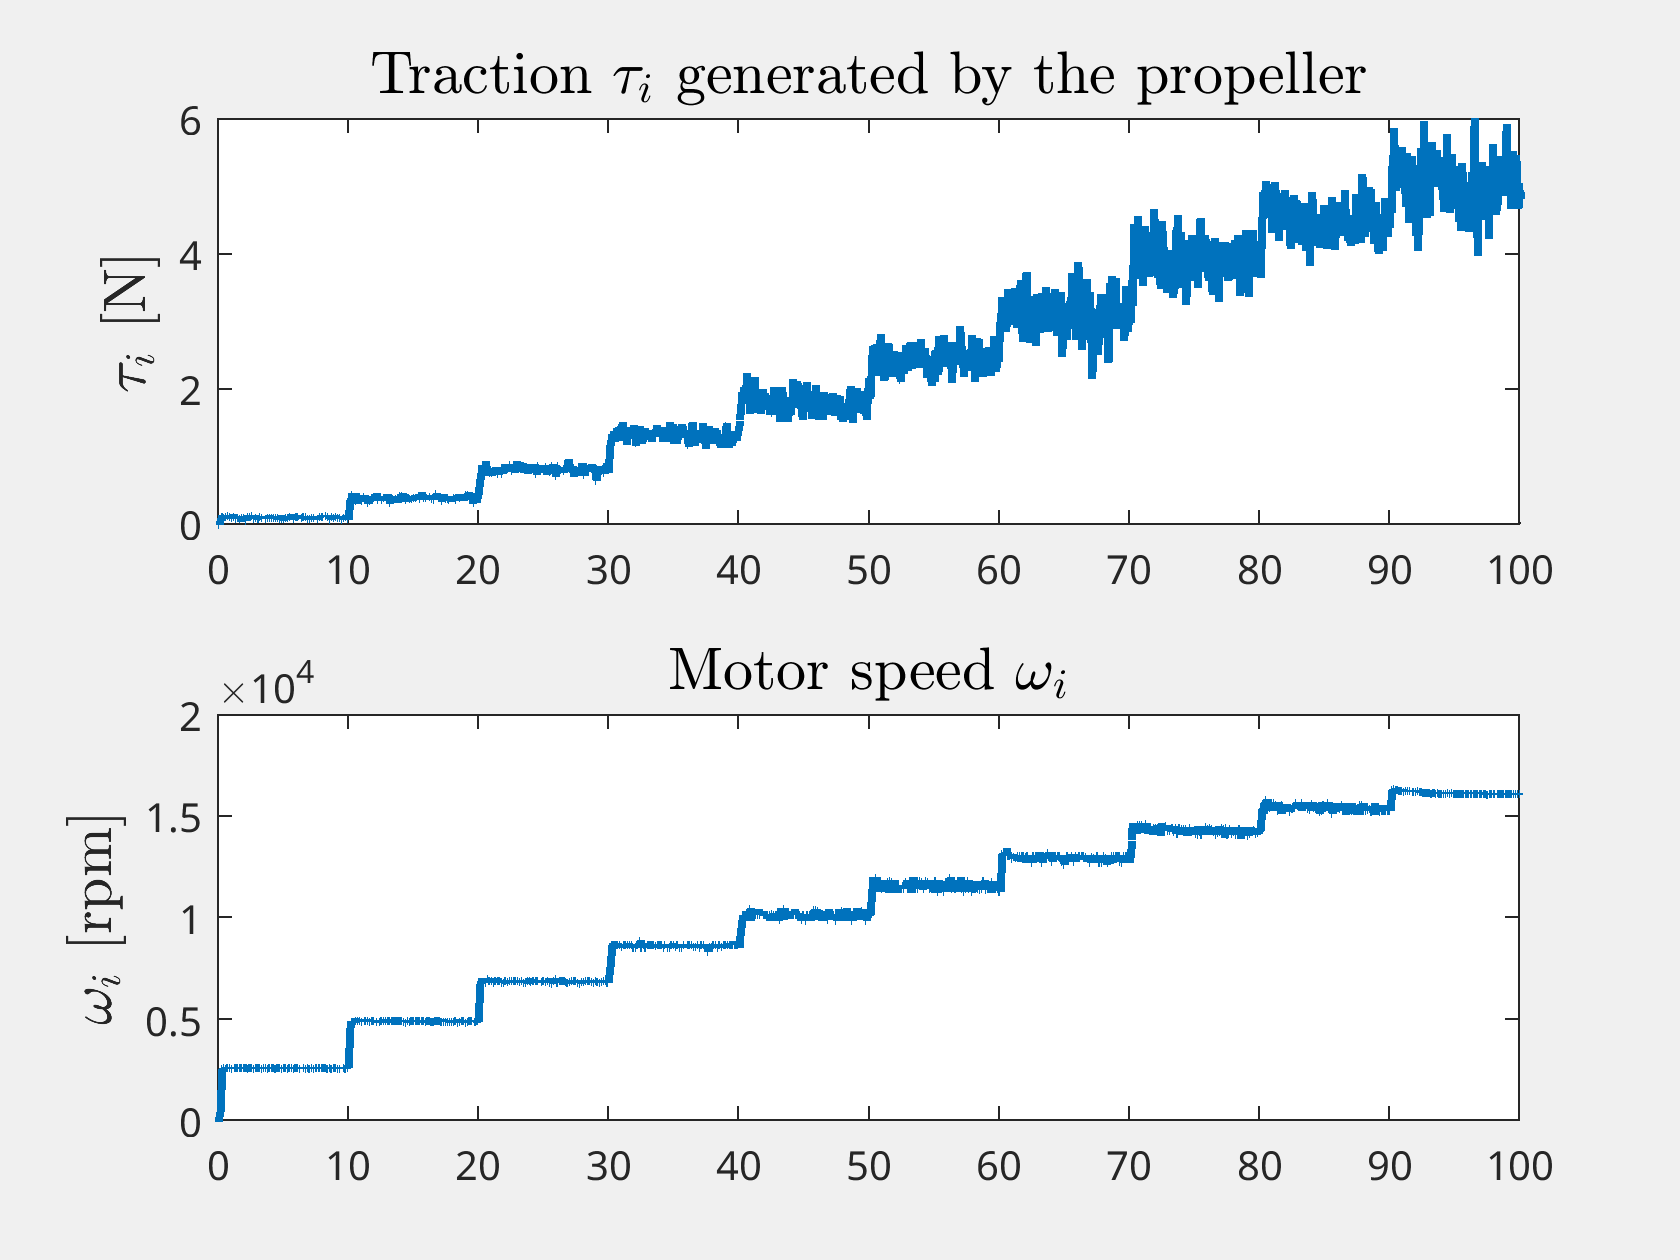
\includegraphics[trim=0cm 0cm 0cm 0cm,clip,width=0.5\columnwidth]{figures/ident_motor March 27 2024 1651.png}}
        \caption{Réponse entrée-sortie de l'ensemble moteur/hélice.}
        \label{fig:IOmot}
    \end{figure}
    
    Pour effectuer l'identification des trois coefficients principaux (diagonaux) de la matrice d'inertie, nous avons réalisé un montage de pendule bifilaire. Cette méthode est largement utilisée dans le domaine des drones \cite{Jardin2007OptimizedMO}, et est basée sur la période d'oscillation autour de chacun des trois axes ($x_{{\text{b}}}$, $y_{\text{b}}$, $z_{\text{b}}$) du drone, lequel est suspendu par deux fils, ce qui forme un pendule de torsion comme le montre la Fig. \ref{fig:BifilarPend}.

    \begin{figure}[ht!]
        \centerline{
        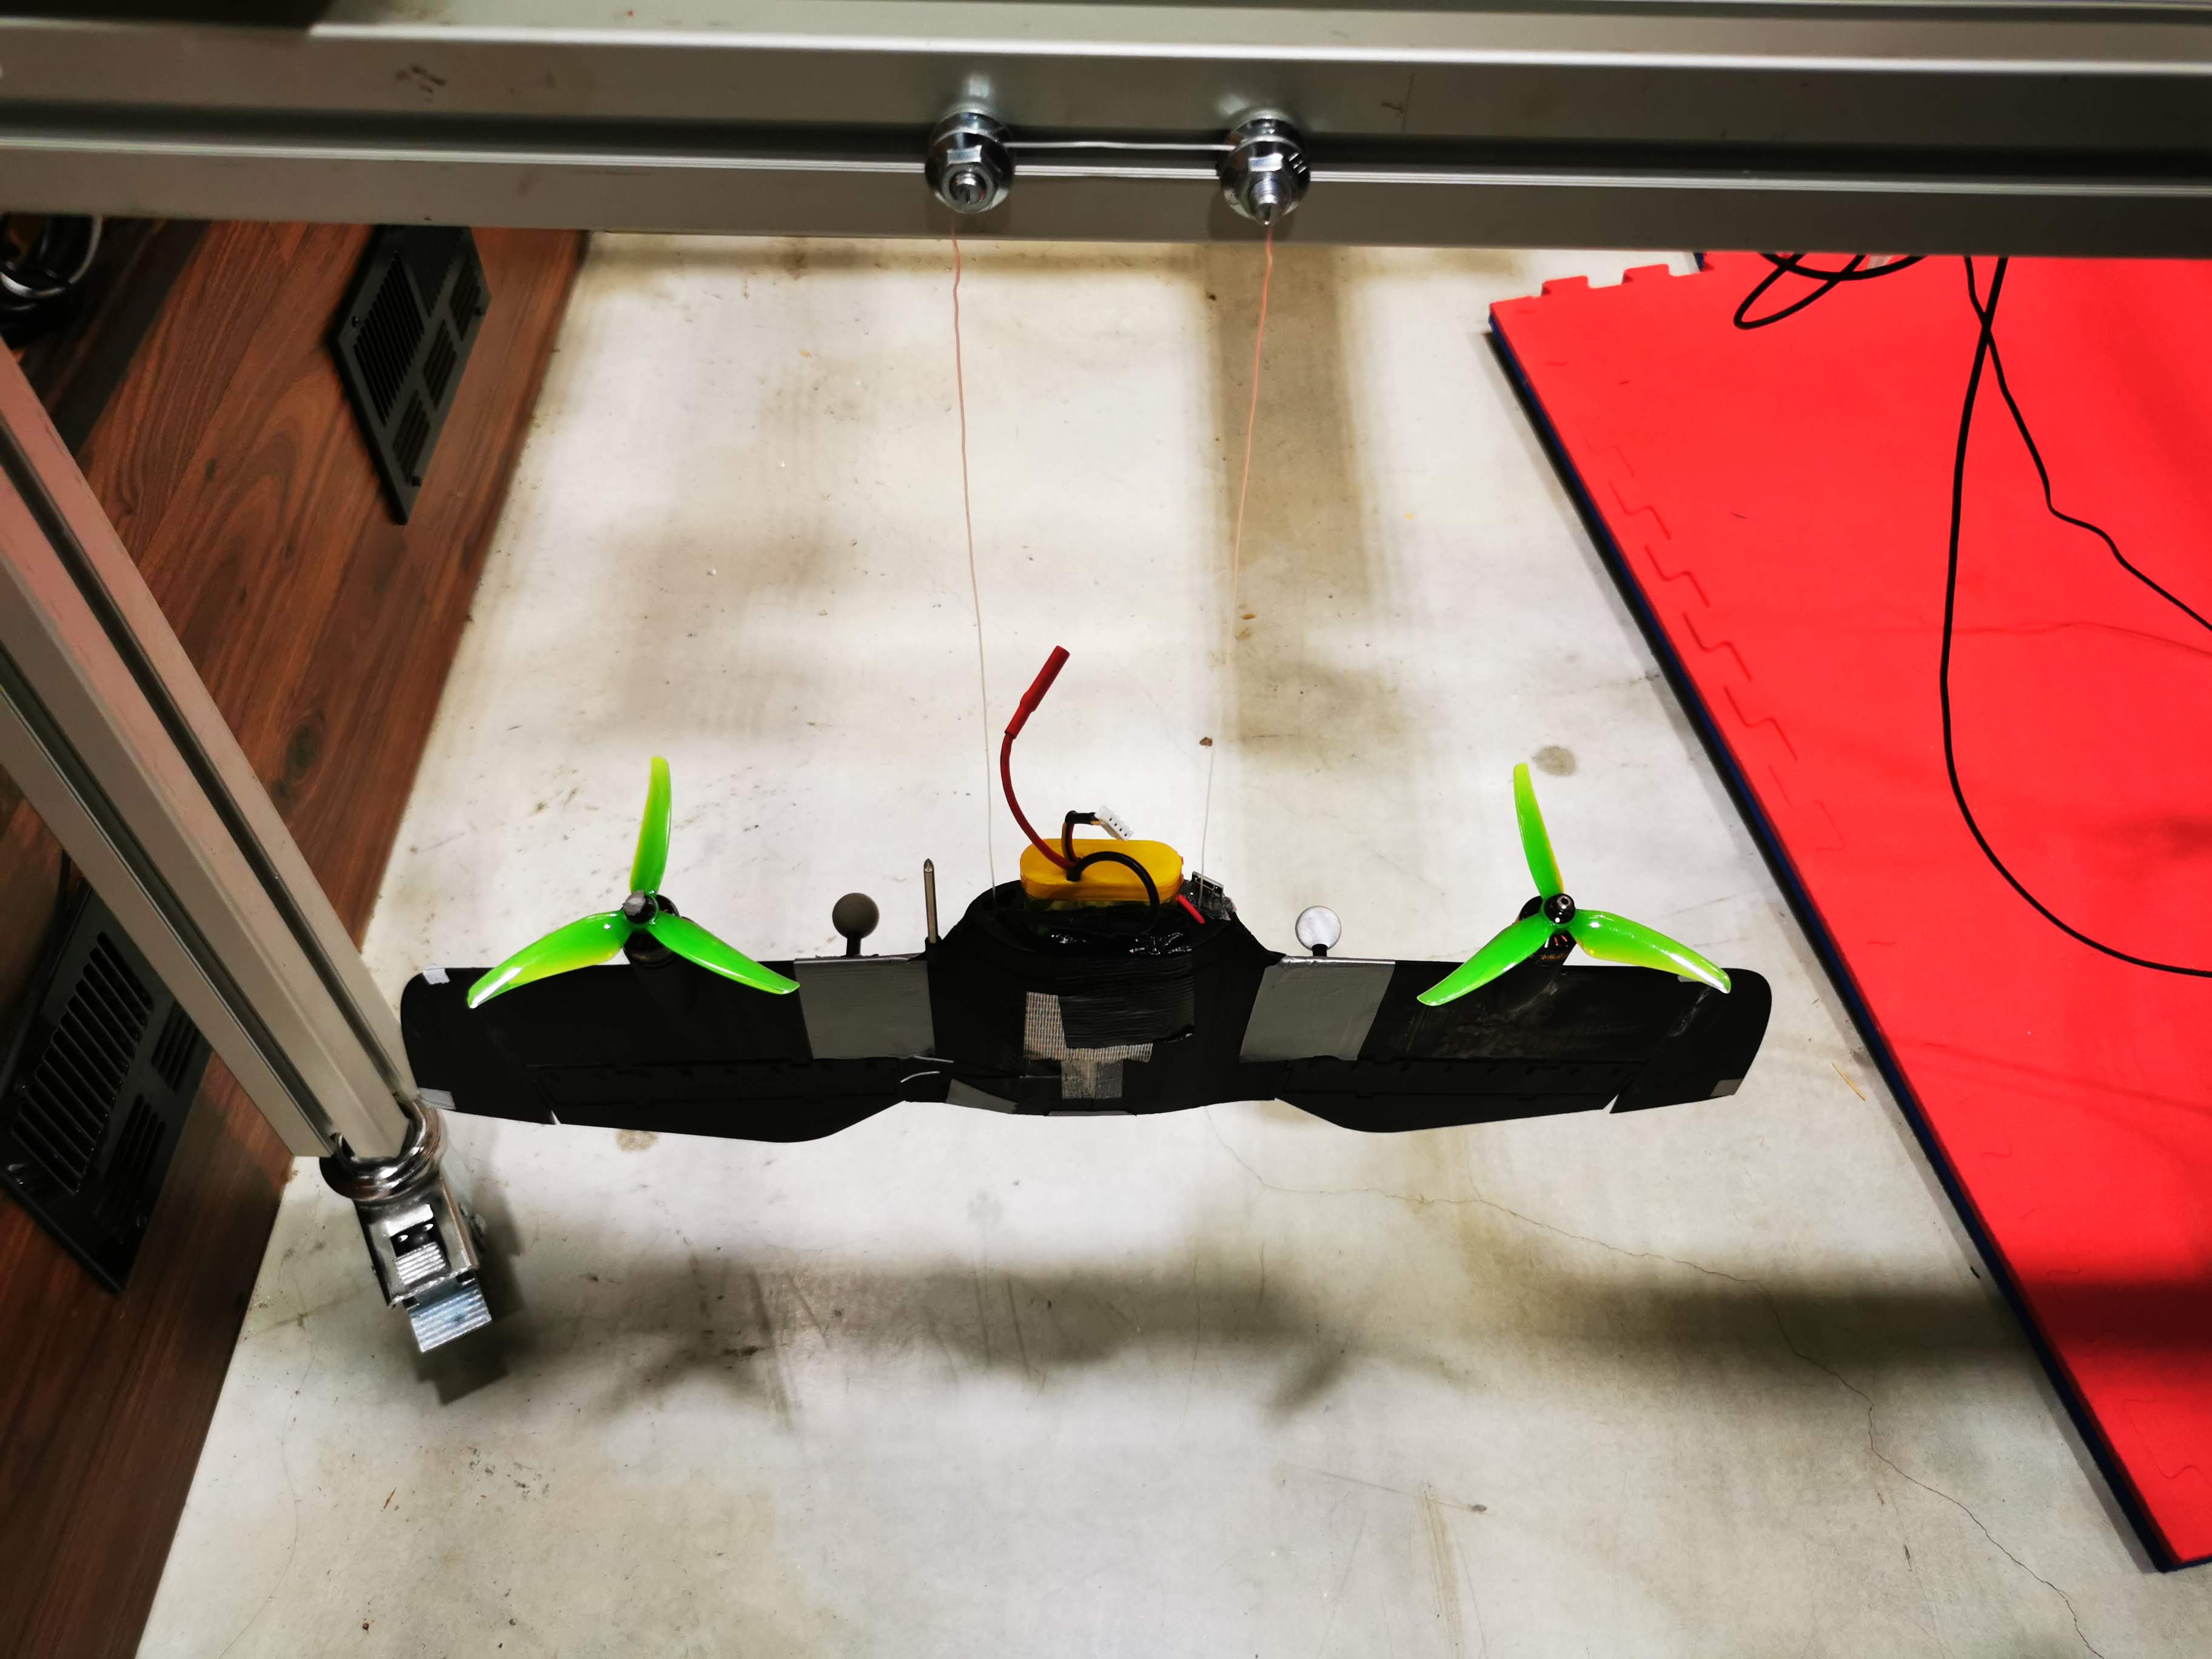
\includegraphics[trim=20cm 15cm 23cm 0cm,clip,width=0.3\columnwidth]{figures/IMG_20230609_085023.jpg}}
        \caption{Montage d'un pendule bifilaire pour l'identification de l'inertie ($\boldsymbol{J}$) de DarkO.}
        \label{fig:BifilarPend}
    \end{figure}

    Lors de la mesure, l'autopilote est utilisé pour réaliser une acquisition de l'orientation du drone à 500 Hz. Le drone est positionné avec un angle non nul vis-à-vis de la position d'équilibre du pendule bifilaire puis il est lâché sans vitesse initiale. Le couple de rappel engendré par les deux fils produit des oscillations amorties (Voir la figure \ref{fig:BifilarPend_meas}). Il est nécessaire de connaître la longueur des fils $h$ ainsi que leur écartement $D$ pour réaliser l'identification. Ces valeurs sont mesurées directement sur le banc de mesure pour chacune des trois configurations et reportées dans la table \ref{tab:lgFils}.

    \begin{table}[ht]
        \centering
        \begin{tabular}{|c|c|c|}
            \hline
             & $h$ & $D$  \\
            \hline\hline
            $J_{x}$ & \SI{0.962}{\meter}  & \SI{0.142}{\meter}  \\
            \hline 
            $J_{y}$ & \SI{0.415}{\meter}  & \SI{0.051}{\meter}  \\
            \hline
            $J_{z}$ & \SI{1.018}{\meter}  & \SI{0.149}{\meter} \\
            \hline
        \end{tabular}
        \caption{Longueur ($h$) et espacement ($D$) des fils du pendule pour chacun des axes.} 
        \label{tab:lgFils}
    \end{table}

    Une fois la mesure réalisée, nous utilisons l'outil \textit{Simulink Design Optimization} pour obtenir les valeurs de l'amortissement visqueux $C$, et de l'inertie sur l'axe mesuré $I$, à partir du modèle suivant :
    \begin{align*}
        \ddot{\theta} +  \frac{C}{I}\dot{\theta} + \left(\frac{mgD^2}{4Ih}\right)\frac{\sin\theta}{\sqrt{1 - 0.5\left(\frac{D}{h}\right)^2(1 - \cos\theta)}} = 0
    \end{align*}
    où $\theta$ est l'angle mesuré par l'autopilote à l'aide du code d'estimation d'état utilisant le gyroscope, l'accéléromètre et l'Optitrack.
    

    \begin{figure}[ht!]
    \centerline{
    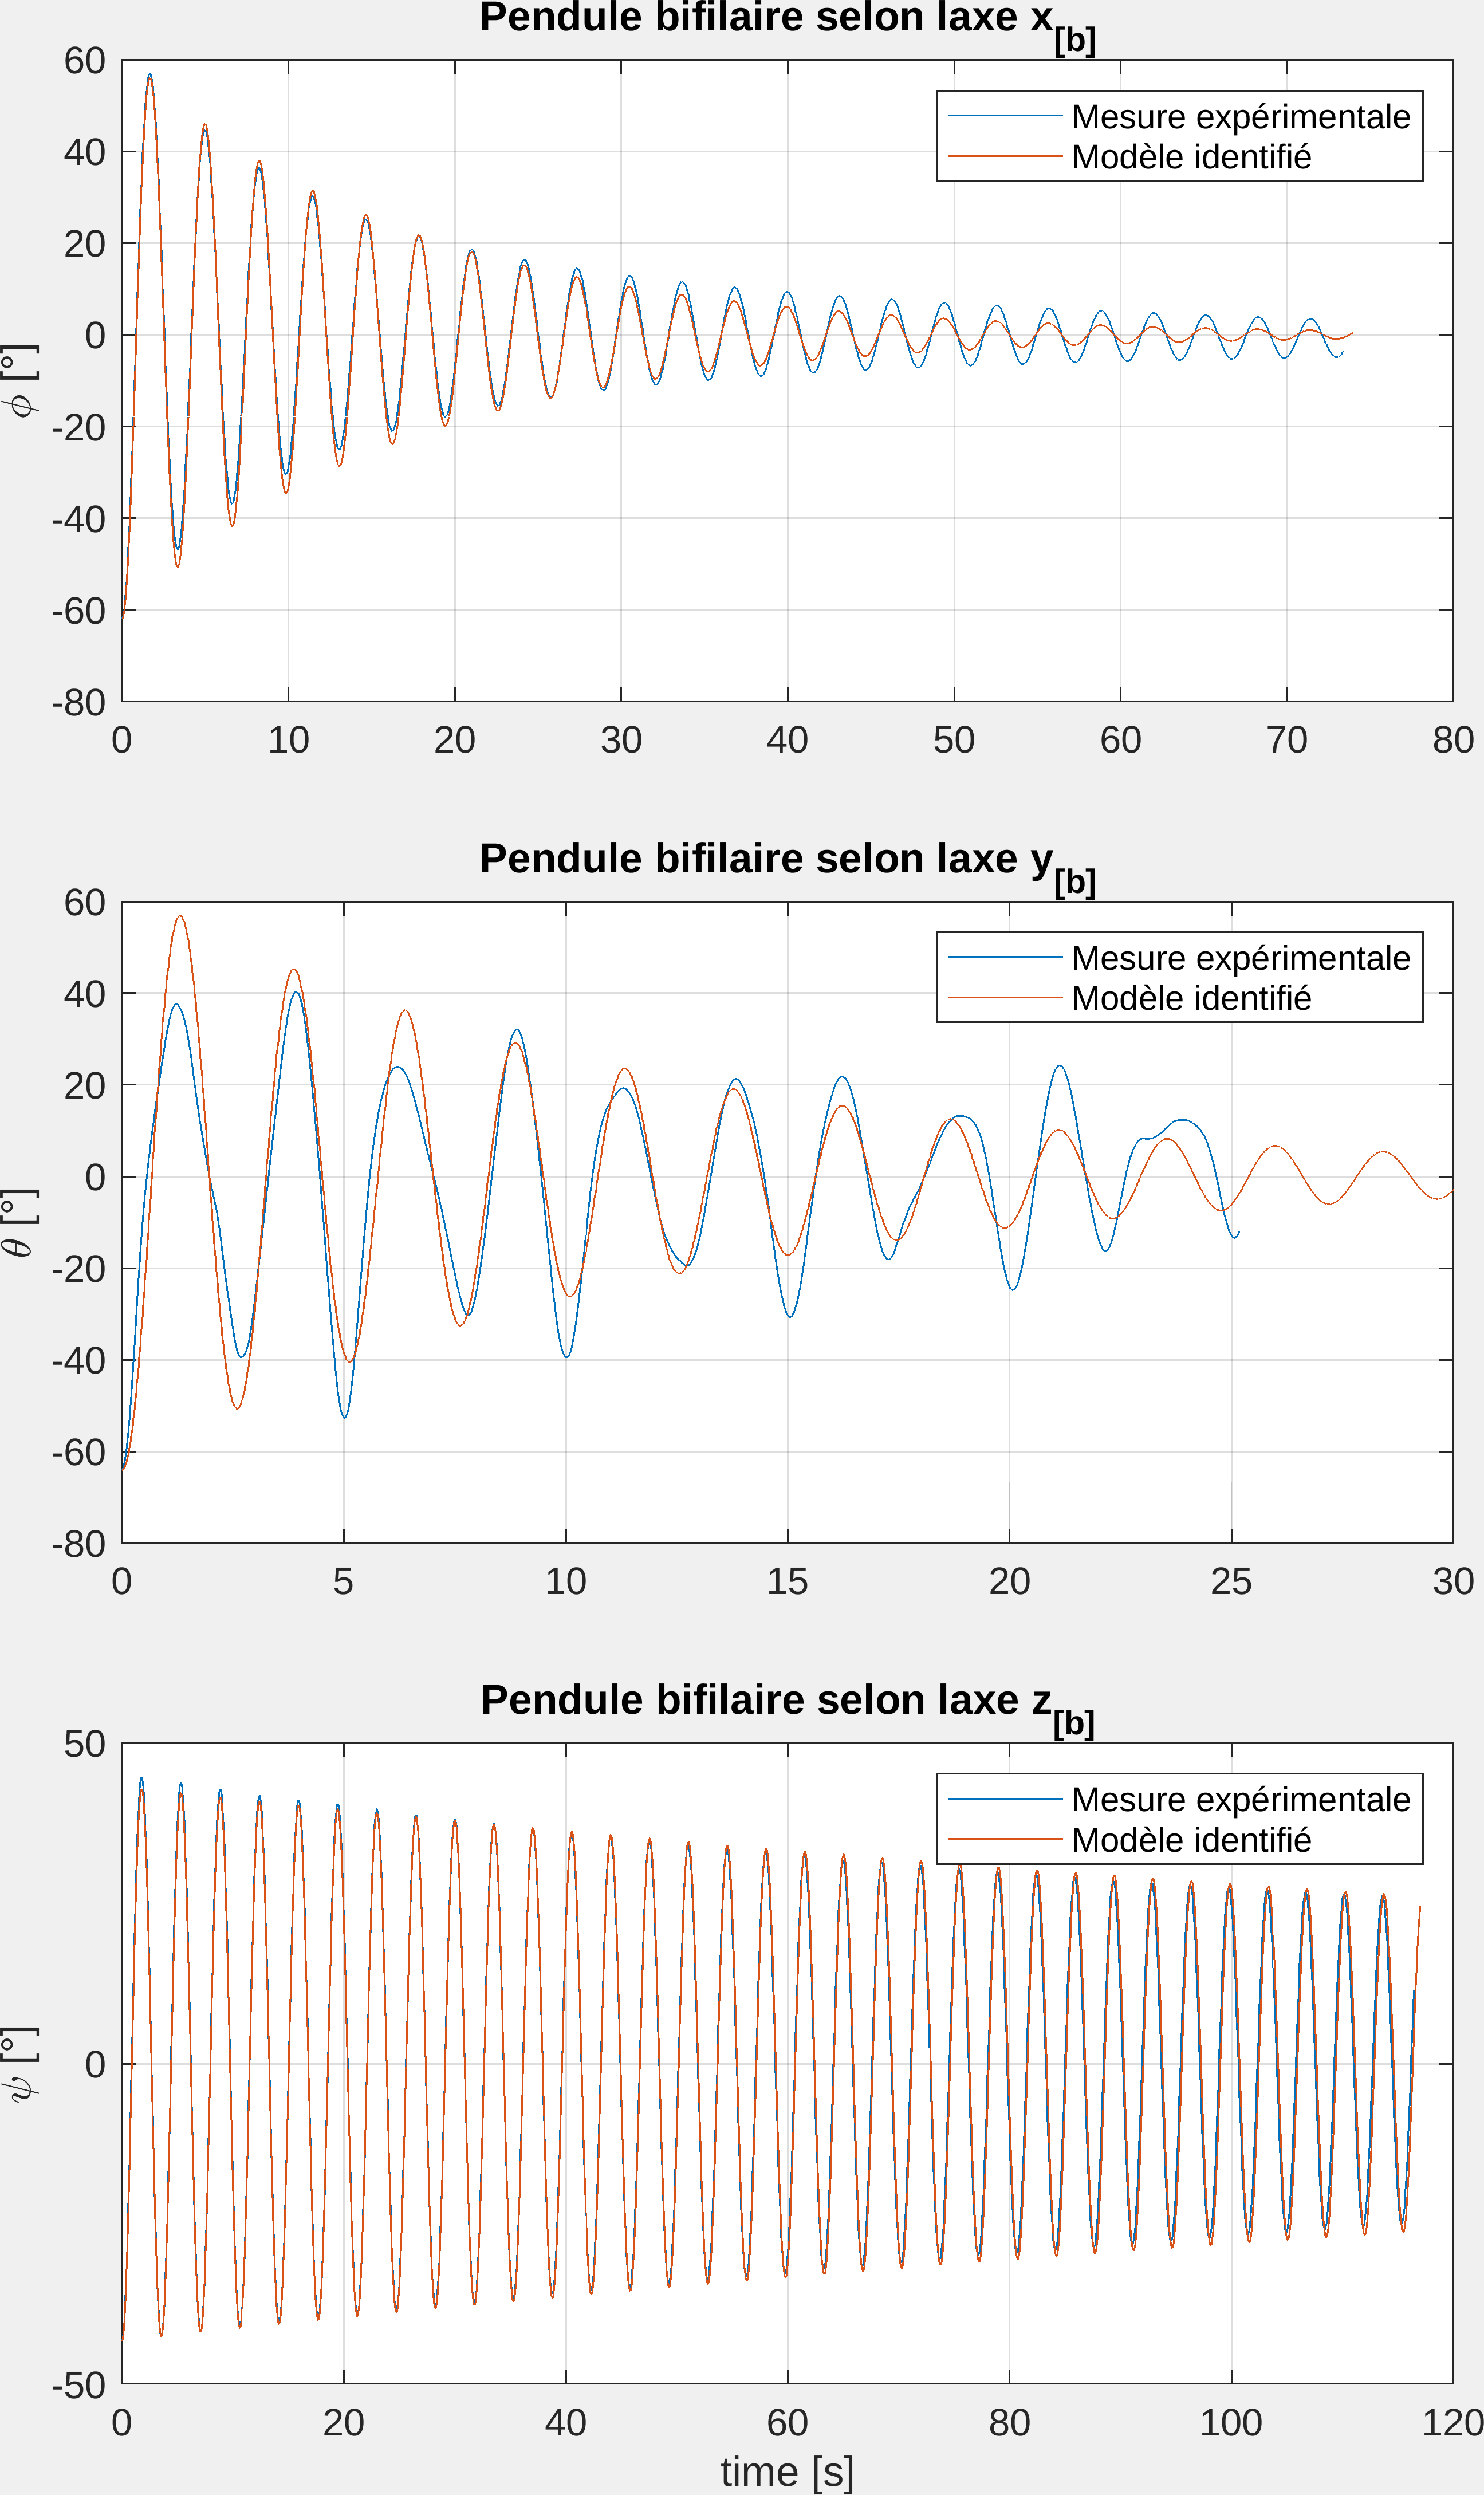
\includegraphics[trim=0cm 0cm 0cm 0cm,clip,width=0.5\columnwidth]{figures/ident_inertia.png}}
    \caption{Identification de l'inertie ($\boldsymbol{J}$), à partir des mesures issues du pendule bifilaire \ref{fig:BifilarPend}.}
    \label{fig:BifilarPend_meas}
    \end{figure}


    
    Les autres coefficients ont été estimés à l'aide d'un montage sur un capteur de forces et moments à 6 degrés de liberté (DOF), observé sur la Figure~\ref{fig:BifilarPend_meas}. \nomenclature[]{\(DOF\)}{Degrés de liberté  (\textit{Degrees of Freedom})}
    \begin{figure}[ht!]
        \centering
        \resizebox{.9\textwidth}{!}{%
        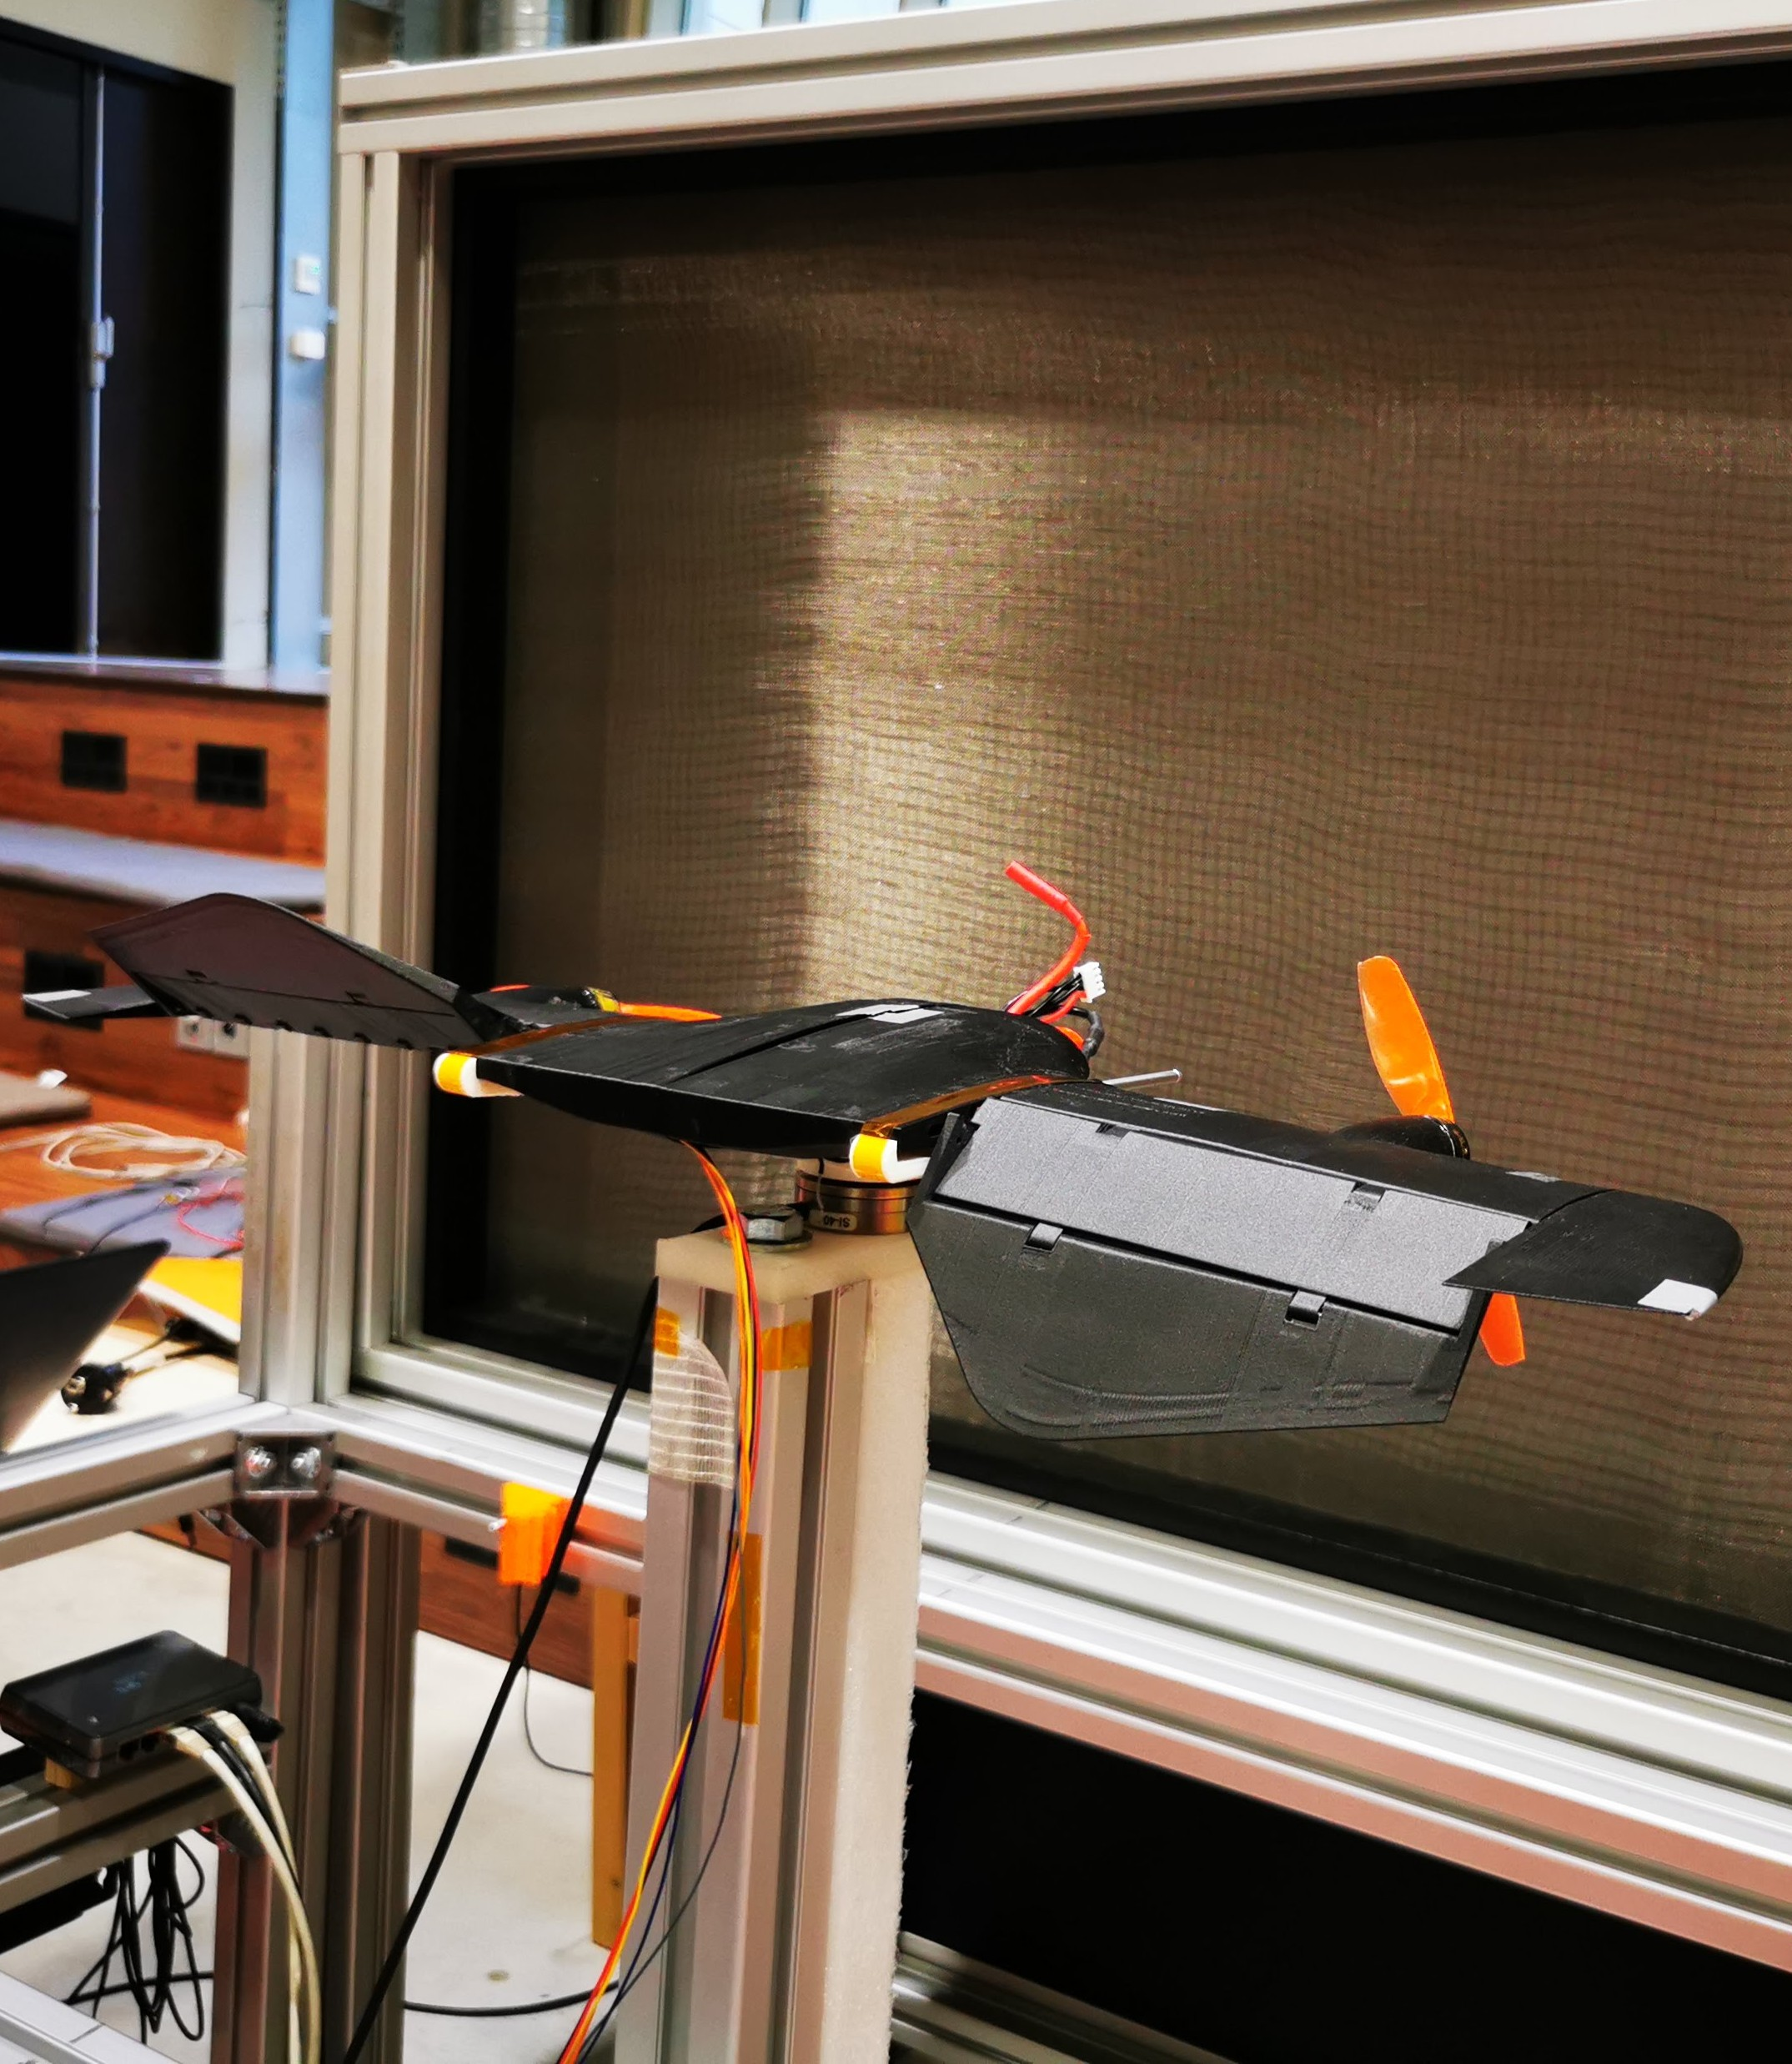
\includegraphics[height=2.5cm]{figures/montage_ident_arr.jpg}
        \quad
        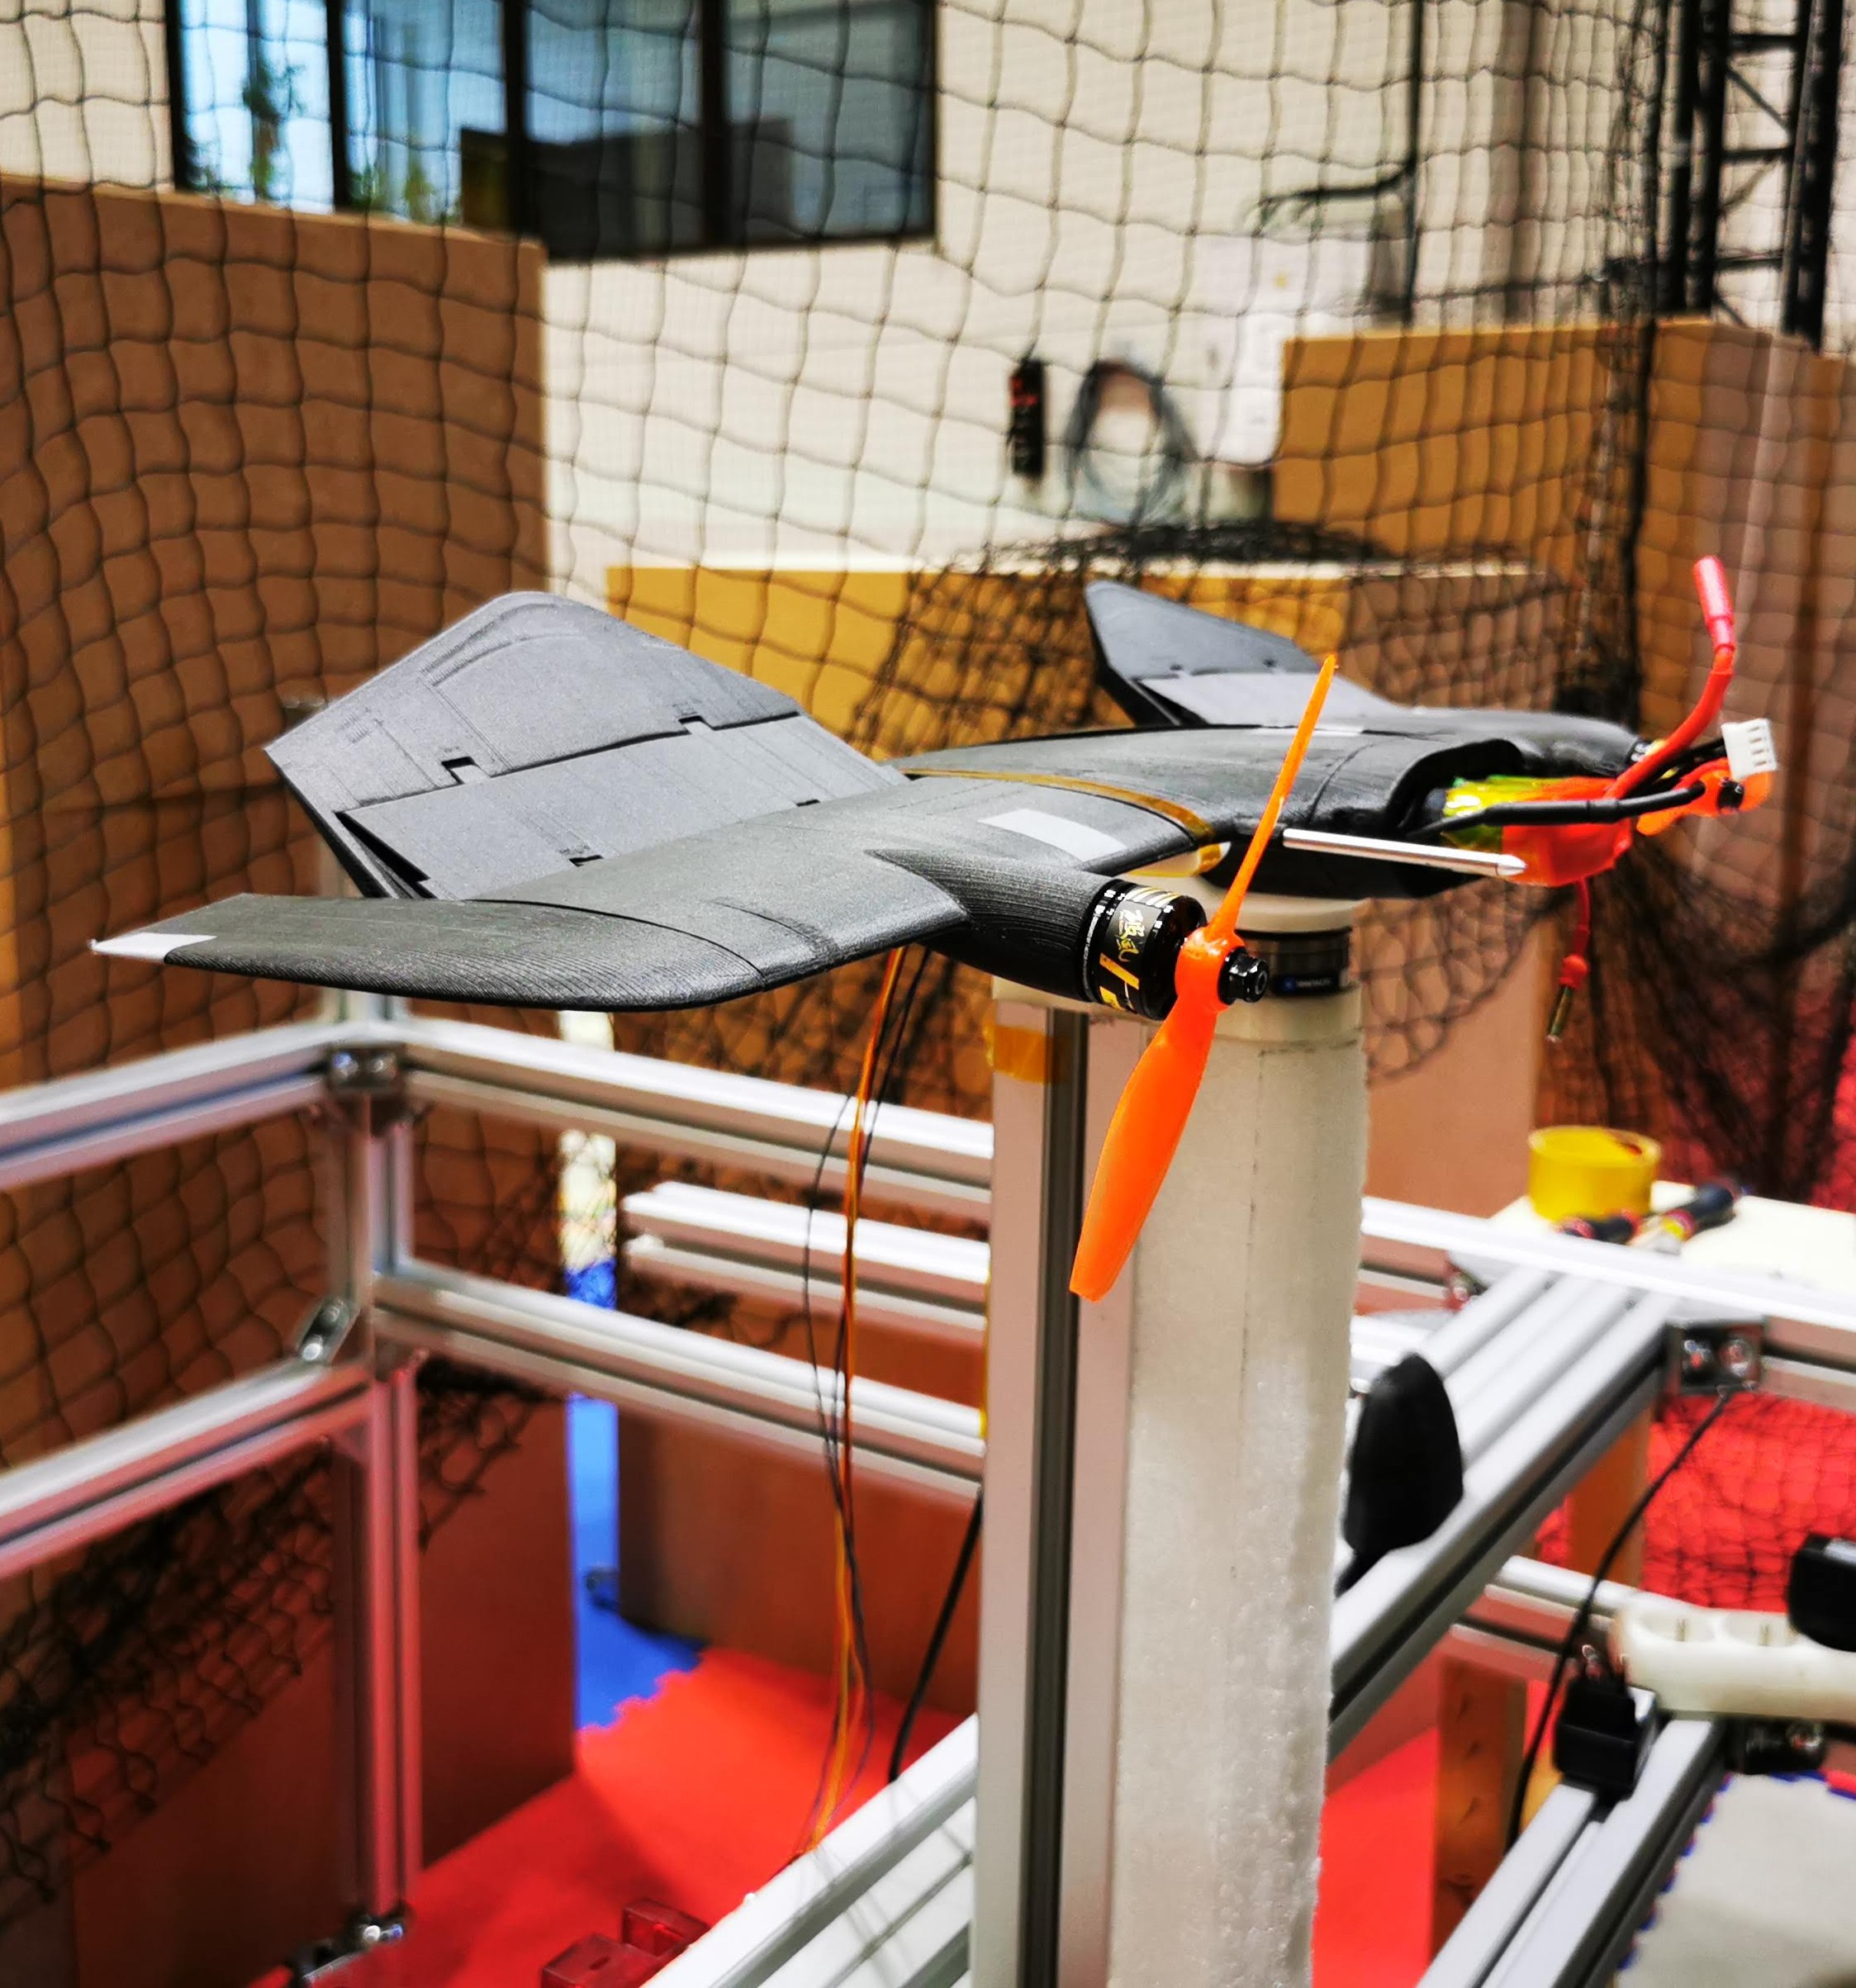
\includegraphics[height=2.5cm]{figures/montage_ident_face.jpg}
        }
        \caption{Montage de DarkO sur un banc de mesure face à une soufflerie ouverte.}
        \label{fig:montage_ident}
    \end{figure}

    Ces mesures permettent d'estimer la surface soufflée par les hélices. Il est intéressant de noter que cette surface représente 67 \% de la surface totale du drone.
    

\subsection{Modélisation des actionneurs}
    \label{sec:saturation}
    Les actionneurs de DarkO ont des dynamiques qui limitent leur action en termes d'amplitude et de vitesse.

    Pour les moteurs électriques générant la traction par les hélices, il existe deux causes de saturation. Une saturation à haute vitesse liée à  la tension maximale du moteur et une saturation basse vitesse liée à la vitesse minimale de commutation de bobine du moteur, pour maintenir la rotation. De plus, ces saturations permettent d'obtenir un modèle réaliste à énergie finie. Elles correspondent à la contrainte suivante : $\omega_i \in [2500,~16000]~rpm = [262,~1675]~\SI{}{\radian\per\second}$, $i=1,2$.
    
    En termes de dynamique, nous avons représenté la chaîne d'actionnement du moteur (composée de l'ESC, du moteur et de l'hélice) par une fonction de transfert du premier ordre ayant une constante de temps égale à \SI{0,0125}{\second}, ce qui fournit un système d'actionnement assez agressif. Cette constante de temps a pu être identifié lors du montage présenté sur la figure \ref{fig:montage_ident}, nous avons piloté un démarrage des moteurs et mesurer la génération de force par le capteur.

    Les saturations impactant les élevons proviennent des limites physiques des servomoteurs et du débattement limité par la forme de l'UAV, $\delta_i \in [-30~; 30]\text{\textdegree}$, $i=1,2$. La contrainte la plus importante, ici, est la bande passante de l'actionneur (due à l'actionnement du servomoteur), qui est modélisée par une fonction de transfert du premier ordre avec une constante de temps \SI{0,05}{\second}. 

\section{Équilibres stationnaires}
\label{sec:eqpoint}
{\color{blue}
    Notre travail a pour point de départ les travaux réalisé par \cite{ olszaneckibarthHal-02542982, smeurINDITail} qui utilise des lois de commande basée mesure. Ces lois de commande fournissent de très bonne propriété de stabilisation même en présence de perturbation. Toutefois, elles permettent d'atteindre des équilibres qui n'ont jamais été caractérisé. Ce manque engendre une incompréhension des mécanismes en jeu lors de déstabilisation. Effectivement, les expérimentations réalisées avec un bouclage INDI ont montré une oscillation de DarkO pour certaines vitesses de vent horizontal. Ainsi, il se pose la question de savoir si ce comportement est dû à un cycle limite lié à des saturations d'actionneur ou bien à des effets aérodynamiques. Pour répondre à cette question, nous allons étudier l'ensemble des points d'équilibre du drone soumis ou non à du vent.
}
    \subsection{Équilibre stationnaire sans vent}
        \label{sec:eq_nowind}

        Nous proposons une modification du vecteur de commande, dans le cas d'un équilibre sans vent $\boldsymbol{w}_{\mathrm{eq}} = 0$, basé sur le couplage des actionneurs. 
        \begin{align}
            \label{eq:vector_u_nowind}
            \boldsymbol{u}_{\text{nowind}} := \begin{bmatrix}\tau_{1}  \!&\! \tau_{2}  \!&\! \delta_{1}\tau_{1} \!&\! \delta_{2}\tau_{2} \end{bmatrix}^\top
        \end{align}
        Nous soulignons que le vecteur $\boldsymbol{u}_{\text{nowind}}$ dans \eqref{eq:vector_u_nowind} correspond à une transformation non inversible des actionneurs de DarkO correspondant à $\boldsymbol{u} := \begin{bmatrix}\tau_{1}  \!&\! \tau_{2}  \!&\! \delta_{1} \!&\! \delta_{2} \end{bmatrix}^\top$ (\eqref{eq:vector_u}). Néanmoins, si l'on impose les contraintes de saturation décrites dans la section~\ref{sec:saturation}, il est possible de déterminer de manière unique $\boldsymbol{u}$ à partir d'une valeur souhaitée de $\boldsymbol{u}_{\text{nowind}}$ dans \eqref{eq:vector_u_nowind}. Les valeurs positives non nulles de $\tau_{1}$ et $\tau_{2}$ peuvent être déterminées à partir des deux premières composantes de $\boldsymbol{u}_{\text{nowind}}$, puis $\delta_1$ et $\delta_2$ sont facilement construites à partir des deux dernières composantes de $\boldsymbol{u}_{\text{nowind}}$. 

        Nous obtenons un modèle linéaire vis-à-vis de sa commande, dérivé de \eqref{eq:dyna_simp} en imposant  $\boldsymbol{w} = 0$,
        \begin{subequations}\label{eq:withouwind}
        \begin{align}
                \boldsymbol{\dot p} &=  \boldsymbol{v}, \quad &
                m\boldsymbol{\dot v} &= - m\boldsymbol{g} +  \boldsymbol{R}(\boldsymbol{q})\boldsymbol{F}\boldsymbol{u}_{\text{nowind}},\\
                \boldsymbol{\dot q} &= \frac{1}{2}\boldsymbol{q} \otimes \smallmat{0 \\ \boldsymbol{\omega}_{\text{b}}} \quad & \boldsymbol{J} \boldsymbol{\dot \omega}_{\text{b}} &= \! \shortminus \skewsym{\boldsymbol{\omega}_{\text{b}}}\!J\boldsymbol{\omega}_{\text{b}} \! + \! \boldsymbol{M}\boldsymbol{u}_{\text{nowind}},
        \end{align}
        \end{subequations}
        avec les matrices :
        \begin{align}
            \label{eq:FandM}
            \left[ \begin{array}{c|c}\!\boldsymbol{F}\!&\!\boldsymbol{M}\!\end{array} \right] := \left[ \begin{array}{cccc | cccc} a_{\text{f}} & a_{\text{f}} & 0 & 0 & a_{\text{m}} & -a_{\text{m}} & b_{\text{m}} & -b_{\text{m}} \\  0 & 0 & 0 & 0 & 0 & 0 & c_{\text{m}} & c_{\text{m}} \\ 0 & 0 & b_{\text{f}} & b_{\text{f}} & d_{\text{m}} & -d_{\text{m}} & 0 & 0 \end{array} \right]
        \end{align}
        et les scalaires :
            \begin{align*}
                \left[\!\! \begin{array}{c|c} 
                a_{\text{f}} & b_{\text{f}} \\ \hline
                a_{\text{m}} & b_{\text{m}} \\ \hline
                c_{\text{m}} & d_{\text{m}}
                \end{array} \!\!\right] \!=\!
                \left[\begin{array}{c|c}
                1-\frac{S_{\text{wet}}}{4S_{\text{p}}} C_{\text{d}}  & -\frac{S_{\text{wet}}}{4S_{\text{p}}}C_{\ell}\xi_{\text{f}} \\ \hline
                \frac{k_{\text{m}} }{k_{\text{f}}}  &   \! \frac{S_{\text{wet}}}{4S_{\text{p}}}a_{y}C_{\ell}\xi_{\text{f}} \!\\ \hline
                \!\! \frac{S_{\text{wet}}}{4S_{\text{p}}} \Delta_{\text{r}}C_{\ell}\xi_{\text{m}} \!\! & 
                p_{y}+\frac{S_{\text{wet}}}{4S_{\text{p}}} a_{y} C_{\text{d}}
                \end{array}\right].
            \end{align*}


        Tous les couples d'équilibre $(\boldsymbol{u}_{\text{nowind}}, \boldsymbol{x}) = (\boldsymbol{u}_{\text{nowind},\text{eq}}, \boldsymbol{x_{\text{eq}}})$ sont paramétrés par une rotation arbitraire autour de l'axe $z_{[\text{i}]}$, définit par $\beta \in \left[-\sqrt{\frac{1}{2}},\sqrt{\frac{1}{2}}\right]$. Le point d'équilibre a pour expression :
        \begin{subequations}
            \label{eq:equilibria}
            \begin{align}
                \label{eq:bar_u}
                \boldsymbol{u}_{\text{nowind},\text{eq}} = \frac{mg}{( 1-\frac{S_{\text{wet}}}{4S_{\text{p}}} C_{\text{d}})} [1~1~0~0]^\top\\
                \boldsymbol{q}_{\text{eq}} = [\eta_{\text{eq}} ~\boldsymbol{\epsilon}_{\text{eq}}^\top]^\top = \smallmat{\sqrt{\frac{1}{2}-\beta} & \beta & \frac{2\beta^{2}-1}{2\sqrt{\frac{1}{2}-\beta}} & \beta}^\top.
            \end{align}
        \end{subequations}
        En présence d'un vent nul, le degré de liberté $\beta$ permet d'orienter le drone dans n'importe quelle direction horizontale.

    \subsection{Équilibre stationnaire en présence de vent}
    \label{sec:eq_vent}
    À partir des modèles \eqref{eq:dyna_orig} et \eqref{eq:dyna_simp}, nous caractérisons un équilibre stationnaire en présence d'un vent constant $\boldsymbol{w}_{\mathrm{eq}} =\smallmat{w_x \\ w_y \\w_z} \in \real^3$ exprimé dans le repère inertiel, tel que $\smallmat{w_x \\ w_y} \neq 0$, c'est-à-dire qu'il existe toujours un vent horizontal non nul.
    Ainsi, pour chaque position de référence $\boldsymbol{p}_{\text{eq}} \in \real^3$, un ensemble de couples état/commande possible est $(\boldsymbol{u}_{\text{eq}}, \boldsymbol{x}_{\text{eq}}) = (\boldsymbol{u}_{\text{eq}}, \boldsymbol{p}_{\text{eq}}, \boldsymbol{v}_{\text{eq}}, \boldsymbol{q}_{\text{eq}}, \boldsymbol{\omega}_{\text{b},\text{eq}})$
    obtenu à l'aide de
    \begin{subequations}
    \label{eq:equilibrium}
    \begin{align}
    \label{eq:ueq}
            &\boldsymbol{u}_{\text{eq}} = \begin{bmatrix} \tau & \tau & \delta & \delta \end{bmatrix}^\top\\
            & \boldsymbol{q}_{\text{eq}} = \boldsymbol{q}_{\mathrm{eq}\psi} \otimes  \boldsymbol{q}_{\mathrm{eq}\theta} \label{eq:qeq}\\
            &\boldsymbol{\omega}_{\text{b},\text{eq}} = 0 , \quad \boldsymbol{v}_{\text{eq}} = 0.
    \end{align}
    \end{subequations}
    Nous définissons deux quaternions $\boldsymbol{q}_{\mathrm{eq}\psi}$ et $\boldsymbol{q}_{\mathrm{eq}\psi}$ permettant d'exprimer l'ensemble des conditions de vent dans le repère inertiel vers un repère tourné où le vent est toujours contenu dans le plan $x-z$. Grâce à cette transformation, nous exprimons un ensemble continu d'équilibres en présence de vent. 

    \begin{align}
    \label{eq:qtheta}
        \boldsymbol{q}_{\mathrm{eq}\theta} &:= \begin{bmatrix} \cos(\frac{\theta}{2}) & 0 & \sin(\frac{\theta}{2}) & 0 \end{bmatrix}^\top
    \end{align}
    \begin{align}
    \label{eq:qpsi}
        \boldsymbol{q}_{\mathrm{eq}\psi} &:= \begin{bmatrix} \cos(\frac{\psi}{2}) & 0 & 0 & \sin(\frac{\psi}{2}) \end{bmatrix}^\top.
    \end{align}
    Les paramètres de l'équilibre sont la rotation horizontale $\psi = \arctan(w_{x}, w_{y})$, l'angle d'inclinaison $\theta$, la poussée des hélices $\tau$, et la déflexion des élevons $\delta$. Ils peuvent être obtenus à partir de l'algorithme~\ref{alg:eq}. 

    \begin{algorithm}
        \caption{Obtention des paramètres d'équilibre en \eqref{eq:equilibrium}.}
        \label{alg:eq}
        \hspace*{.1cm} \textbf{Entrée} : Vecteur vent $\boldsymbol{w}_{\text{eq}} =\smallmat{w_x & w_y & w_z}^\top$ \\
        \hspace*{.1cm} \textbf{Sortie} : Paramètres $\psi$, $\theta$, $\tau$, $\delta$ dans \eqref{eq:equilibrium}
        \begin{algorithmic}[1]
            %\Require {\bf Input} values: $\boldsymbol{w} =\smallmat{w_x & w_y & w_z}^\top$ 
            %\Ensure  $\psi$, $\theta$, $\tau$, $\delta$
            \State Détermine l'angle $\psi = \text{atan2}(w_x, w_y)$ de manière à obtenir $\boldsymbol{q}_{\mathrm{eq}\psi}$ dans \eqref{eq:qpsi}  
            \State Détermine la perturbation tournée $\boldsymbol{w}_{\text{r}}$ avec la composante $y$ nulle, en utilisant $\boldsymbol{R}_{\psi}:= \smallmat{ \cos \psi & \sin \psi & 0 \\ -\sin \psi & \cos \psi & 0 \\ 0 & 0 & 1 }$, selon :
            \begin{align}
            \label{eq:wh}
            \boldsymbol{w}_{\mathrm{r,eq}} := \smallmat{w_{\text{r}x} \\ 0 \\w_{\text{r}z}} :=  \boldsymbol{R}^\top(\boldsymbol{q}_{\mathrm{eq}\psi}) \boldsymbol{w}_{\mathrm{eq}} = \boldsymbol{R}^\top_{\psi} \boldsymbol{w}_{\mathrm{eq}}
            \end{align}

            \State Détermine l'angle d'inclinaison $\theta$ de manière à obtenir $\boldsymbol{q}_{\text{eq}\theta}$ dans \eqref{eq:qeq}:  
            \begin{align}
            \label{eq:theta_alg}
                \theta = -\tan^{-1}\left(\frac{w_{\text{r}z}}{w_{\text{r}x}} + \frac{2mg}{\rho S \lVert \boldsymbol{w}_{\mathrm{eq}} \rVert C_{\ell}  (1-\frac{\xi_{\text{f}}}{\xi_{\text{m}}}) w_{\text{r}x} } \right)
            \end{align}
        \State Pour des raisons de commodité, nous définissons les scalaires :
            $$ 
            \left[\begin{array}{c|c} 
            \!\!a\!\!&\!\!b\!\! \\ \hline \!\!c\!\!&\!\! d\!\!\end{array}  \right] \!:=\! 
            \left[\begin{array}{c|c}
            2 S_{\text{wet}} C_{\ell} mg \sin{\theta} \xi_{\text{f}} &
            \! 2 S_{\text{wet}} C_{\text{d}} C_{\ell} \rho  \lVert \boldsymbol{w}_{\mathrm{eq}} \rVert  w_{x}^{\text{b}}\!\! \\ \hline
            \!\!-4 S S_{\text{p}} C_{\ell} \rho  \lVert \boldsymbol{w}_{\mathrm{eq}} \rVert  w_{x}^{\text{b}} \xi_{\text{f}}\!\! & \frac{b \xi_{\text{f}}}{2}
            \end{array}\right]
            $$ 
            et grâce à ces scalaires $(a,b,c,d)$, déterminons la traction des hélices $\tau$ dans \eqref{eq:ueq} comme :
            \begin{align}
                \nonumber
                \tau &= \frac{S_{\text{p}}}{2 S_{\text{wet}} C_{\ell} \xi_{\text{f}} (4S_{\text{p}} -  S_{\text{wet}} C_{\text{d}} )} \Bigg( a+b+c+d + \Bigg[ (a+b+c \shortminus d)^2 \shortminus 4 (d^2+ac \shortminus bd)  \\ 
                & \quad
                \shortminus \frac{4 {w_{z}^{\text{b}}}^2 d}{ {w_{x}^{\text{b}}}^2 } (d+c) + \frac{4 w_{z}^{\text{b}}ad\cos{\theta}}{w_{x}^{\text{b}} C_{\ell} \sin{\theta} } \left(C_{\text{d}} - \frac{4 S_{\text{p}}}{S_{\text{wet}}}\right) \Bigg] ^{\frac{1}{2}} \Bigg),\label{eq:tau_alg}
            \end{align}
            où
            $$
            \bigmat{w_{x}^{\text{b}} \\ w_{z}^{\text{b}}} = \bigmat{   w_{\text{r}x} \cos{\theta} - w_{\text{r}z} \sin{\theta}\\
                        w_{\text{r}x} \sin{\theta} +  w_{\text{r}z} \cos{\theta} }.
            $$
            
            \State Déterminons la déflexion des élevons $\delta$ comme :
            \begin{align}
            \label{eq:delta_alg}
                \delta = \frac{2mg\sin{\theta}}{\rho S \lVert \boldsymbol{w}_{\mathrm{eq}} \rVert C_{\text{d}}\xi_{\text{f}} w_{z}^{\text{b}}} + \frac{w_{x}^{\text{b}}}{\xi_{\text{f}}w_{z}^{\text{b}}} -  \frac{(4-\frac{S_{\text{wet}}}{S_{\text{p}}} C_{\text{d}})}{\rho S \lVert \boldsymbol{w}_{\mathrm{eq}} \rVert C_{\text{d}}\xi_{\text{f}} w_{z}^{\text{b}}} \tau.
            \end{align}

        \end{algorithmic}
        \hspace*{.1cm} \textbf{Retourne}:  $\psi$, $\theta$, $\tau$, $\delta$
    \end{algorithm}

    \noindent\begin{minipage}{\linewidth}
        \begin{theorem}\label{thm:eqs}
        Pour tout vent constant, $\boldsymbol{w} =\smallmat{w_x & w_y & w_z}^\top \in \real^3$ ayant une composante horizontale non nulle $\smallmat{w_x \\ w_y}$, les équations \eqref{eq:qpsi}--\eqref{eq:qtheta} avec $\theta$, $\tau$ et $\delta$ sélectionnées selon l'Algorithme~\ref{alg:eq} caractérisent un couple d'équilibre $(\boldsymbol{u}_{\text{eq}}, \boldsymbol{x}_{\text{eq}})$ pour la dynamique non linéaire \eqref{eq:dyna_orig} et \eqref{eq:dyna_simp}.
        \end{theorem}
    \end{minipage}
    
    \begin{proof}
        Dans un premier temps, notons qu'avec l'expression de $\boldsymbol{R}$ \eqref{eq:matrix_rot} et l'expression de  $\psi$ dans l'étape 1 de l'Algorithme~\ref{alg:eq}, on peut définir la perturbation à l'équilibre tournée $\boldsymbol{w}_{\mathrm{r,eq}} := \boldsymbol{R}^\top_{\psi} \boldsymbol{w}_{\mathrm{eq}} :=    \boldsymbol{R}^\top(\boldsymbol{q}_{\mathrm{eq}\psi})\boldsymbol{w}_{\mathrm{eq}}$ (voir \eqref{eq:wh} dans l'Algorithme~\ref{alg:eq}), correspond à la rotation nécessaire pour aligner l'axe  $x_{[\text{b}]}$ du repère corps avec la direction du vent. Une fois que le drone est face au vent, il subit un vent avec une composante latérale $y$ nulle et peut ajuster son angle d'inclinaison $\theta$ afin de générer la poussée et la portance nécessaires pour compenser les effets du vent dans les directions longitudinale et verticale (l'effet latéral est nul en raison de l'orientation spécifique de l'appareil $\psi$). Avec cette rotation $\psi$, il est possible d'exprimer le vent dans le repère corps comme étant :
            \begin{align}
            \label{eq:wb}
                \boldsymbol{w}^{\text{b}}_{\mathrm{eq}} &:= 
                \begin{bmatrix}
                    w_{x}^{\text{b}} \\ 0 \\ w_{z}^{\text{b}}
                \end{bmatrix} \!=\! 
                \boldsymbol{R}^\top(\boldsymbol{q}_{\text{eq}\theta}) \boldsymbol{w}_{\mathrm{r,eq}}  \\
                &=\!\! \begin{bmatrix}
                    \cos{\theta} & 0 & -\sin{\theta}\\
                        0 & 1 & 0\\
                    \sin{\theta} & 0 & \cos{\theta}
                \end{bmatrix}^\top \!\! \begin{bmatrix}
                    w_{\text{r}x}\\
                    0\\
                    w_{\text{r}z}
                \end{bmatrix}
                \!\!=\!\!\begin{bmatrix}
                    w_{\text{r}x} \cos{\theta} - w_{\text{r}z} \sin{\theta}\\
                    0\\
                    w_{\text{r}x} \sin{\theta} +  w_{\text{r}z} \cos{\theta}
                \end{bmatrix}.
            \nonumber
            \end{align}

        Nous insistons sur le fait que $w_{x}^{\text{b}}$ est toujours négatif et différent de zéro, car le drone est orienté dans la direction du vent grâce à la rotation engendrée par $ \boldsymbol{q}_{\mathrm{eq}\psi}$, et suite à l'hypothèse $\smallmat{w_x \\ w_y} \neq 0$.
    
        L'équation \eqref{eq:dyna1} montre qu'il est nécessaire d'avoir $\boldsymbol{v}_{\text{eq}} = 0$ pour maintenir l'équilibre stationnaire. En multipliant \eqref{eq:dyna2} par $\boldsymbol{R}(\boldsymbol{q}_{\text{eq}})$ donnée dans  \eqref{eq:wb}, nous l'exprimons dans le repère corps.
        Comme nous appliquons la même commande $\tau_{1} = \tau_{2} = \tau $ aux deux moteurs et la même commande aux deux élevons $\delta_{1} = \delta_{2} = \delta$, nous obtenons pour les deux modèles \eqref{eq:dyna_orig} et \eqref{eq:dyna_simp}, l'équilibre des forces selon l'axe $x_{[\text{b}]}$ donné par :
        \begin{align}
            & (2-\frac{S_{\text{wet}}}{2S_{\text{p}}} C_{\text{d}})\tau - \frac{1}{2}\rho S \lVert \boldsymbol{w}_{\mathrm{eq}} \rVert C_{\text{d}} \left(w_{x}^{\text{b}} - \xi_{\text{f}} \delta w_{z}^{\text{b}} \right) - mg \sin(\theta) = 0 \label{eq:forcex}
        \end{align}
        et l'équilibre des forces selon l'axe $z_{[\text{b}]}$ donné par : 
        \begin{align}\label{eq:forcez}
            - \frac{S_{\text{wet}}}{2S_{\text{p}}}\xi_{\text{f}} C_{\ell} \tau \delta - \frac{1}{2}\rho S \lVert \boldsymbol{w}_{\mathrm{eq}} \rVert C_{\ell} \left(w_{z}^{\text{b}} + \xi_{\text{f}} \delta w_{x}^{\text{b}} \right) + mg \cos(\theta) = 0.
        \end{align}
        De manière similaire, à partir de \eqref{eq:dyna_orig_d} et \eqref{eq:dyna4}, l'équilibre des moments autour de l'axe $y_{[\text{b}]}$ permet d'obtenir : 
        \begin{align}\label{eq:momenty}
            \frac{S_{\text{wet}}}{2S_{\text{p}}}  \Delta_{\text{r}} \xi_{\text{m}} C_{\ell} \tau \delta + \frac{1}{2}\rho S \Delta_{\text{r}} \lVert \boldsymbol{w}_{\mathrm{eq}} \rVert C_{\ell} \left(w_{z}^{\text{b}} + \xi_{\text{m}} \delta w_{x}^{\text{b}} \right) = 0.
        \end{align}
        
        Pour calculer la solution du triplet ($\theta$,$\tau$,$\delta$) des trois équations d'équilibre \eqref{eq:forcex}--\eqref{eq:momenty}, ajoutons \eqref{eq:forcez} multipliée par $\Delta_{\text{r}} \xi_{\text{m}}$, à \eqref{eq:momenty} multipliée par $\xi_{\text{f}}$, de manière à annuler le premier terme et à obtenir : 
        \begin{multline*}
            \Delta_{\text{r}} \xi_{\text{m}} \left( - \frac{1}{2}\rho S \lVert \boldsymbol{w}_{\mathrm{eq}} \rVert C_{\ell} (w_{z}^{\text{b}} + \xi_{\text{f}} \delta w_{x}^{\text{b}}) + mg \cos(\theta) \right) \\+ \xi_{\text{f}} \left(\frac{1}{2}\rho S  \Delta_{\text{r}} \lVert \boldsymbol{w}_{\mathrm{eq}} \rVert C_{\ell} (w_{z}^{\text{b}} + \xi_{\text{m}} \delta w_{x}^{\text{b}})  \right) = 0,
        \end{multline*}
        qui est équivalent à
        \begin{align*}
            \frac{1}{2}\rho S  \Delta_{\text{r}} \lVert \boldsymbol{w}_{\mathrm{eq}} \rVert C_{\ell}  (\xi_{\text{f}} - \xi_{\text{m}}) w_{z}^{\text{b}} +   \Delta_{\text{r}} \xi_{\text{m}} mg \cos(\theta)  = 0,
        \end{align*}
        où ($w_{x}^{\text{b}}$,$w_{z}^{\text{b}}$) sont les première et troisième composantes de $\boldsymbol{w}^{\text{b}}$ dans \eqref{eq:wb}. Ensuite, en utilisant \eqref{eq:wb} et après calcul, nous obtenons : 
        \begin{multline*}
                -\frac{1}{2}\rho S  \Delta_{\text{r}} \lVert \boldsymbol{w}_{\mathrm{eq}} \rVert C_{\ell}  (\xi_{\text{f}} - \xi_{\text{m}}) w_{\text{r}x} \sin{\theta}  +\bigg( -\frac{1}{2}\rho S  \Delta_{\text{r}} \\ \lVert \boldsymbol{w}_{\mathrm{eq}} \rVert C_{\ell}  (\xi_{\text{f}} - \xi_{\text{m}})w_{\text{r}z} +   \Delta_{\text{r}} \xi_{\text{m}} mg \bigg) \cos{\theta} = 0,
        \end{multline*}
        qui est satisfaite par :
            \begin{align} \label{eq:theta}
                \theta &=  -\tan^{-1}\left(\frac{\rho S \lVert \boldsymbol{w}_{\mathrm{eq}} \rVert C_{\ell}  (\xi_{\text{f}} - \xi_{\text{m}})w_{\text{r}z} - 2 \xi_{\text{m}} mg }{\rho S\lVert \boldsymbol{w}_{\mathrm{eq}} \rVert C_{\ell}  (\xi_{\text{f}} - \xi_{\text{m}}) w_{\text{r}x}}\right).
            \end{align}
        Cette dernière expression coïncide avec la sélection \eqref{eq:theta_alg} dans l'Algorithme~\ref{alg:eq}.
        À partir de \eqref{eq:theta_alg}, nous pouvons calculer les commandes à l'équilibre en substituant \eqref{eq:forcex} dans \eqref{eq:forcez}. Après simplifications, la force nécessaire de traction des hélices  $\tau$ pour maintenir la position d'équilibre correspond à l'expression  \eqref{eq:tau_alg}. Finalement, avec la valeur de $\tau$ dans \eqref{eq:tau_alg}, nous pouvons obtenir la déflexion des élevons nécessaire $\delta$ à partir de l'équation \eqref{eq:forcez}, ce qui nous donne la valeur obtenue dans \eqref{eq:delta_alg}.
    \end{proof}
    Il est intéressant de noter que pour chaque couple de vent($w_{\text{r}z}$, $w_{\text{r}x}$) correspond une orientation d'équilibre \eqref{eq:qeq}, \eqref{eq:theta_alg} étant indépendante de l'entrée $\boldsymbol{u}_{\text{eq}}$. En outre, il convient de souligner que pour toutes les valeurs de vent raisonnables, l'équation \eqref{eq:tau_alg} correspond à la racine positive d'un polynôme du second ordre, l'autre racine étant toujours négative, ce qui conduit à une condition de poussée négative physiquement impossible.


    À partir de l'expression analytique \eqref{eq:equilibrium} de l'équilibre du drone pour différentes conditions de vent $\boldsymbol{w}$, nous reportons, sur la Fig. \ref{fig:saturation}, les valeurs correspondantes de $\theta$, $\delta$, $\tau$ pour des valeurs de vitesse de vent horizontal allant de 0 à \SI{-20}{\meter\per\second} et pour des valeurs de vitesse de vent vertical allant de \SI{-6}{} à \SI{6}{\meter\per\second}. L'angle d'incidence $\theta$ diminue de \SI{90}{\degree} à \SI{-4.65}{\degree}. $\theta = \SI{90}{\degree}$ correspond à un vol stationnaire sans vent. La traction $\tau$ atteint son minimum à $w_{rx} = \SI{-12.8}{\meter\per\second}$, ce qui correspond à une condition de vol qui minimise la consommation d'énergie, car les moteurs sont la principale source de consommation électrique.

    \begin{figure}[ht!]
        \centering
        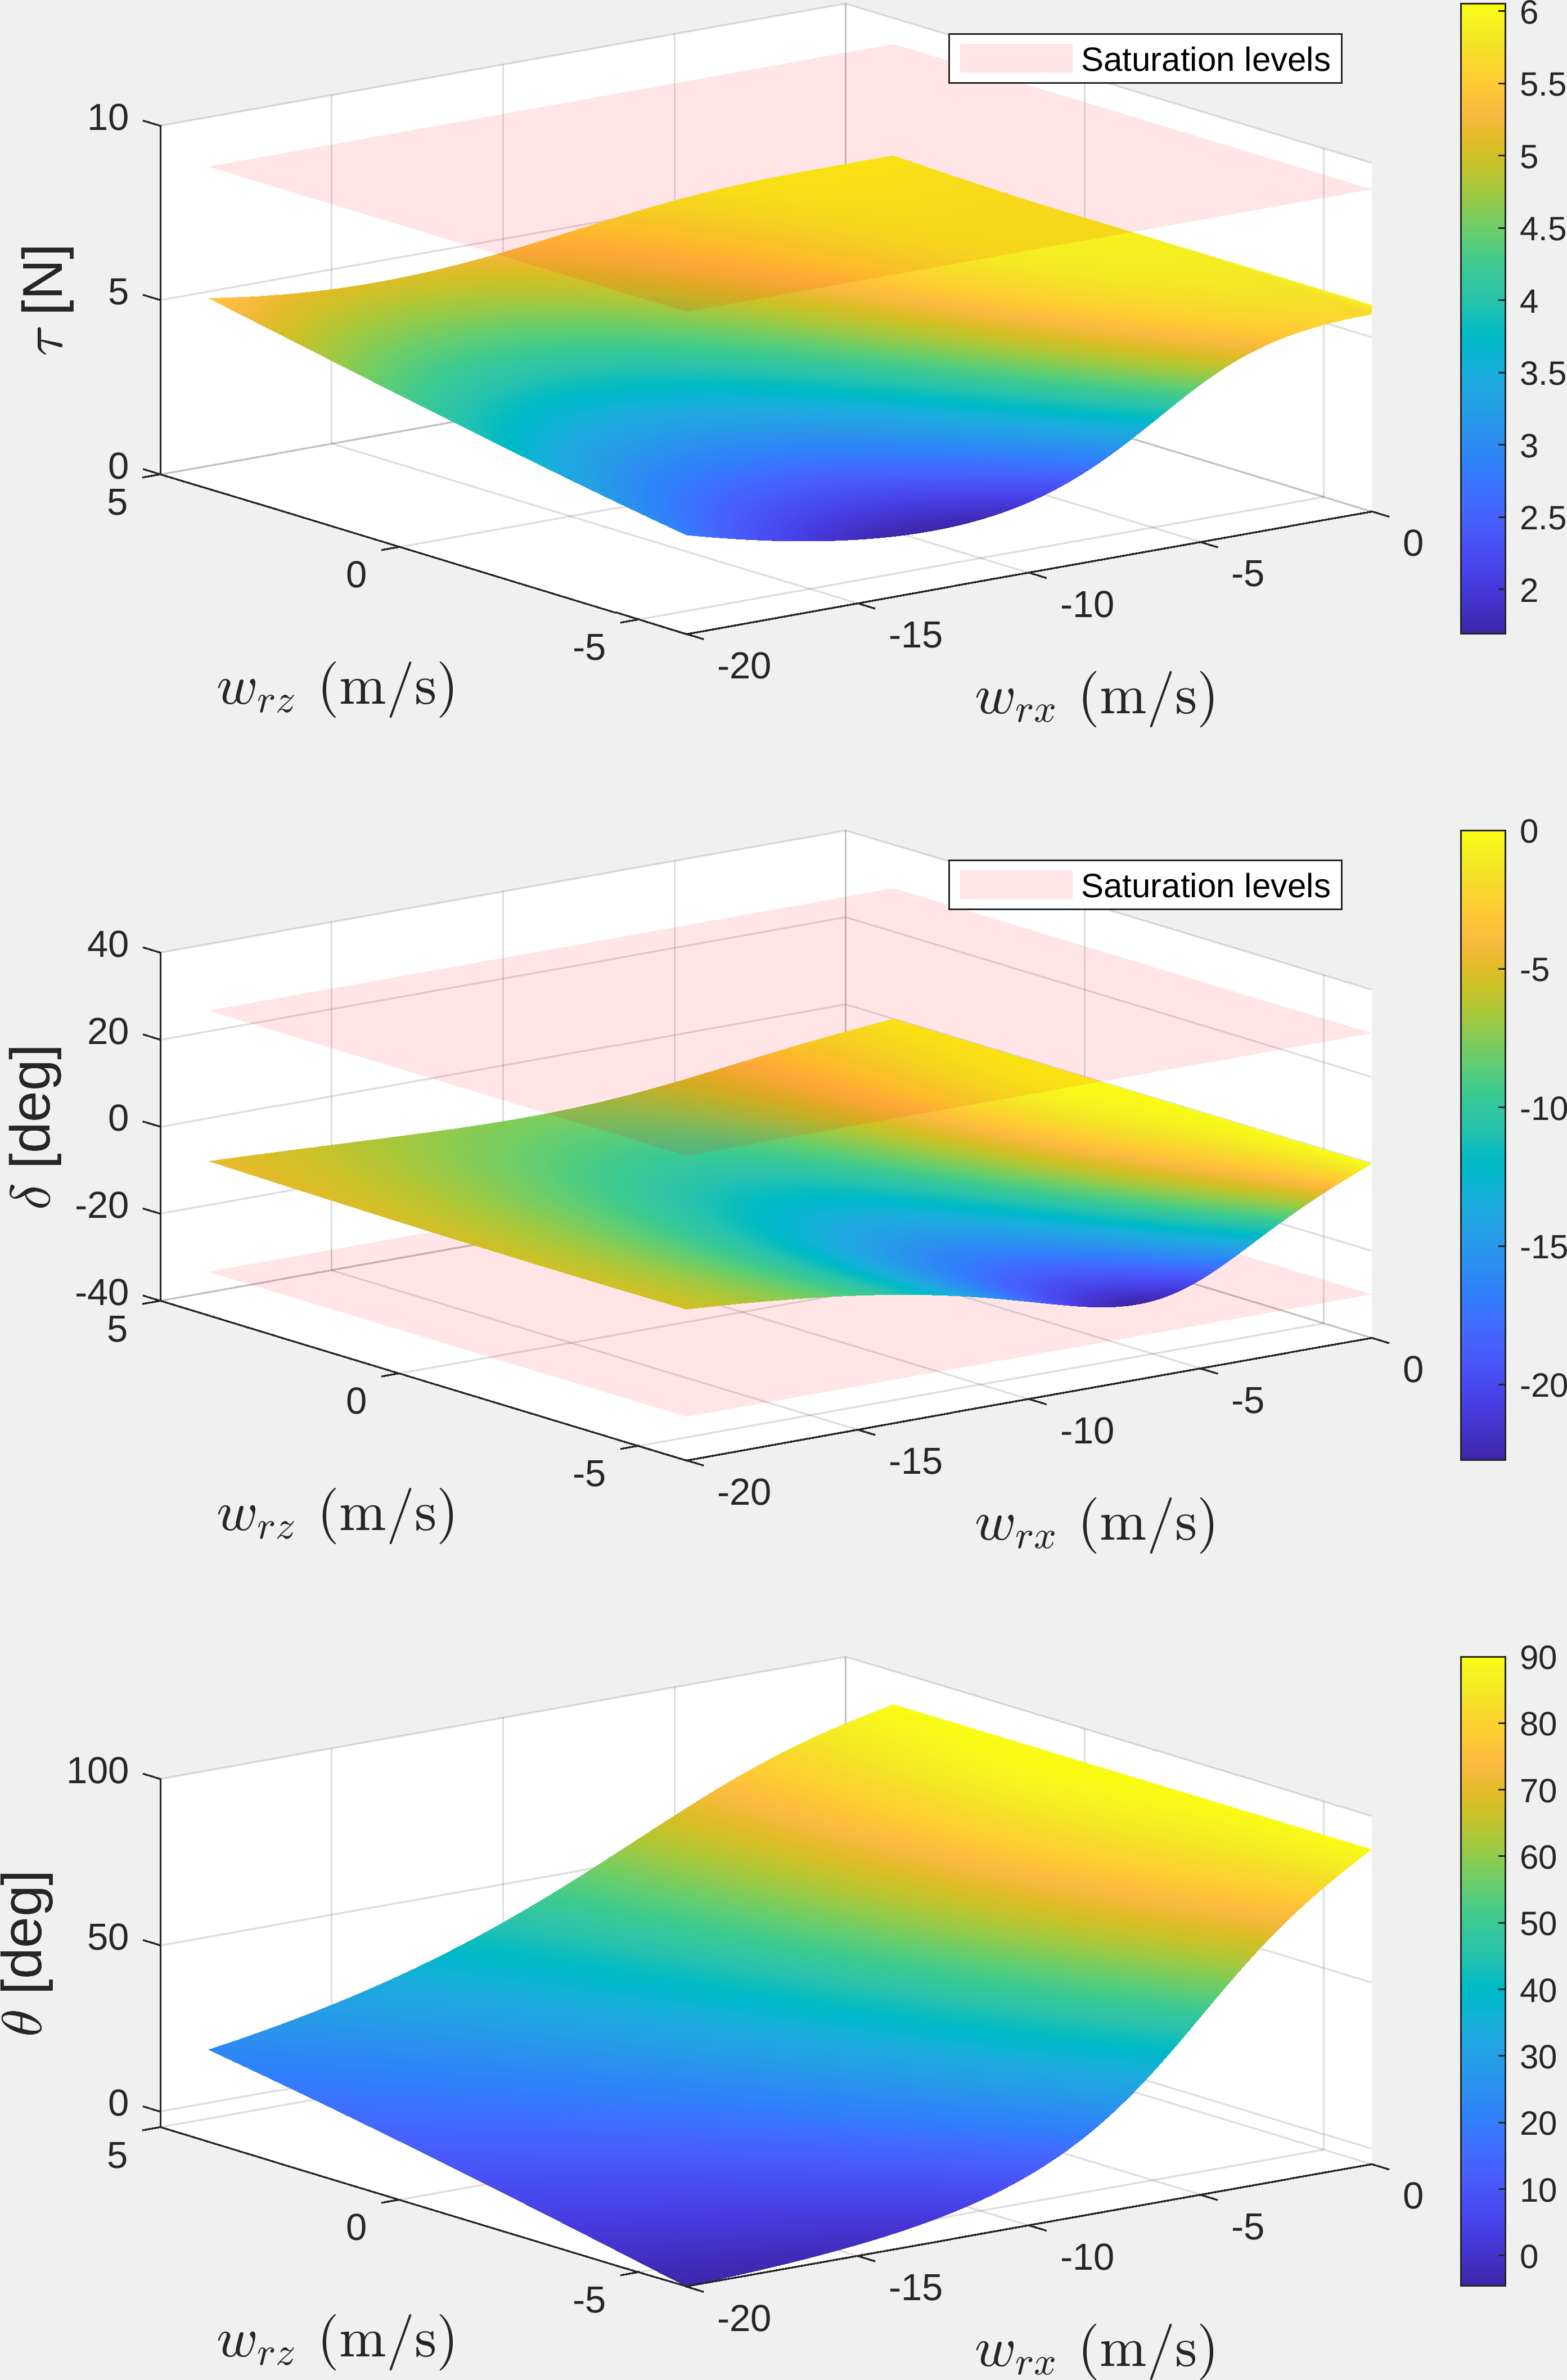
\includegraphics[trim=0cm 0cm 0cm 0cm,clip,width=0.5\columnwidth]{figures/equilibrium_wx_wz.png}
        \caption{Les paramètres ($\tau$, $\delta$, $\theta$) de l'ensemble des points d'équilibre (surface) obtenus à l'aide du Théorème~\ref{thm:eqs} et de l'Algorithme \ref{alg:eq} pour un vent constant horizontal et vertical ($w_{\text{r}x}$,$w_{\text{r}z}$), avec les saturations des actionneurs (rose).}
        \label{fig:saturation}
    \end{figure}
    Il est possible de faire une coupe des surfaces présentées dans \eqref{fig:saturation} pour une vitesse verticale nulle $\boldsymbol{w}_{\text{rx}} = 0$, ce qui nous donne le résultat de la Figure \ref{fig:saturation_wz0}
    \begin{figure}[ht!]
        \centering
        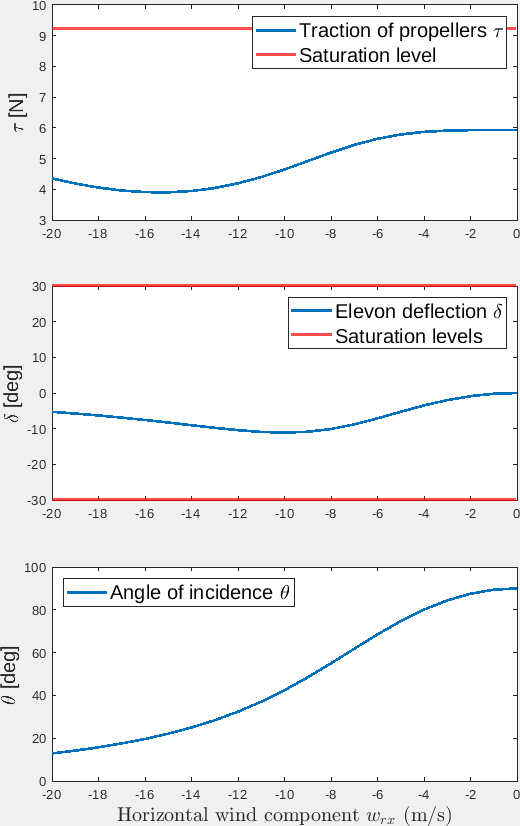
\includegraphics[trim=0cm 0cm 0cm 0cm,clip,width=0.5\columnwidth]{figures/equilibrium.png}
        \caption{Section des surfaces de la Figure \ref{fig:saturation} pour $w_{\text{r}z} = \SI{0}{\meter\per\second}$.}
        \label{fig:saturation_wz0}
    \end{figure}

\section{Dynamiques linéarisées}
{\color{blue}
    Des points équilibres obtenus dans la section \ref{sec:eqpoint} et notamment de l'Algorithme~\ref{alg:eq}, il semble cohérent de poursuivre notre travail en obtenant les dynamiques linéarisés autours des points d'équilibre. Ces résultats permettront, par exemple, de concevoir des lois de commande linéaire basée modèle
}
\subsection{Dynamique linéarisée sans vent}
\label{sec:nowind_lin}
Considérons le cas sans vent discuté dans la section \ref{sec:eq_nowind} pour lequel nous utilisons le vecteur de commande $\boldsymbol{u}_{\text{nowind}}$  et le vecteur de commande à l'équilibre $\boldsymbol{u}_{\text{nowind},\text{eq}}$ défini dans l'équation \eqref{eq:bar_u} et rappelons la transformation du vecteur de commande suivante $ \boldsymbol{u}_{\text{nowind}} := \begin{bmatrix}\tau_{1}  \!&\! \tau_{2}  \!&\! \delta_{1}\tau_{1} \!&\! \delta_{2}\tau_{2} \end{bmatrix}^\top$. La dynamique linéarisée dans le cas sans vent est :
\begin{align}
    \label{eq:linearized}
     \boldsymbol{\dot{\tilde{x}}} = \boldsymbol{A}_{0} \tilde{\boldsymbol{x}} + \boldsymbol{G}_{0} (\boldsymbol{u}_{\text{nowind}}-\boldsymbol{u}_{\text{nowind},\text{eq}}),
\end{align}
où l'expression de $\boldsymbol{A}_{0}$ est : 
\begin{align}
    \label{matrice_A}
        \boldsymbol{A}_{0} = \boldsymbol{A}_{w} \Big|_{\boldsymbol{w}=0} =\begin{bmatrix}
        \mathbb{0}_{3} & \mathbb{I}_{3} & \mathbb{0}_{3} & \mathbb{0}_{3} \\
        \mathbb{0}_{3} & \mathbb{0}_{3} &  \boldsymbol{A}_{v\epsilon} & \mathbb{0}_{3} \\
        \mathbb{0}_{3} & \mathbb{0}_{3} & \mathbb{0}_{3} & \boldsymbol{A}_{\epsilon\omega} \\
        \mathbb{0}_{3} & \mathbb{0}_{3} & \mathbb{0}_{3} & \mathbb{0}_{3}
        \end{bmatrix},
\end{align}
avec les matrices suivantes : 
\begin{align*}
    \boldsymbol{A}_{\epsilon\omega} = \frac{\sqrt{2}}{4}\begin{bmatrix} 
        1 & 0 & -1 \\ 
        0 & 1 & 0  \\
       1 & 0 & 1
    \end{bmatrix} \text{ et } \boldsymbol{A}_{ v\epsilon} = \sqrt{2}\begin{bmatrix} 
        0 & -2g & 0\\
        g & 0 & g  \\ 
         0 & -2g & 0 \end{bmatrix},
\end{align*}
alors que l'expression de $\boldsymbol{G}_{0}$ est :
\begin{align}
    \label{matriceG0}
    \boldsymbol{G}_{0}  := \begin{bmatrix}
    \mathbb{0}_{3\times 1} & \mathbb{0}_{3\times 1} & \mathbb{0}_{3\times 1} & \mathbb{0}_{3\times 1}\\
    0 & 0 & a_{\text{g}} & a_{\text{g}}\\
    0 & 0 & 0 & 0\\
    b_{\text{g}} & b_{\text{g}}  & 0 & 0\\
    \mathbb{0}_{3\times 1} & \mathbb{0}_{3\times 1} & \mathbb{0}_{3\times 1} & \mathbb{0}_{3\times 1}\\
    c_{\text{g}} & -c_{\text{g}} & d_{\text{g}} & -d_{\text{g}}\\
    0 & 0 & e_{\text{g}} & e_{\text{g}}\\
    f_{\text{g}} & -f_{\text{g}} & 0 & 0\\
    \end{bmatrix} , 
\end{align}
avec : 
\begin{align*}
    \left[\!\! \begin{array}{c|c} 
    a_{\text{g}} & b_{\text{g}} \\ \hline
    c_{\text{g}} & d_{\text{g}} \\ \hline
    e_{\text{g}} & f_{\text{g}}
    \end{array} \!\!\right] \!=\!
    \left[\begin{array}{c|c}
   \shortminus \frac{S_{\text{wet}}}{4mS_{\text{p}}}C_{\ell}\xi_{\text{f}}  & \frac{1}{m}( 1-\frac{S_{\text{wet}}}{2S_{\text{p}}} C_{\text{d}}) \\ \hline
    \frac{k_{\text{m}} }{J_{x}k_{\text{f}}}  &   \! \frac{ S_{\text{wet}} a_{y} }{4 J_{x} S_{\text{p}} } C_{\ell}\xi_{\text{f}} \!\\ \hline
    \!\! \frac{S_{\text{wet}}\Delta_{\text{r}}}{4J_{y}S_{\text{p}}} C_{\ell}\xi_{\text{m}} \!\! & 
    \frac{1}{J_{z}}(p_{y}\!+\!\frac{S_{\text{wet}}}{4S_{\text{p}}} a_{y} C_{\text{d}})\!\!
    \end{array}\right].
\end{align*}

\subsection{Dynamique linéarisée en présence de vent}

Pour chacun des équilibres caractérisés dans le Théorème~\ref{thm:eqs}, nous détaillons les équations linéarisées du mouvement par rapport au modèle non linéaire simplifié à faible vitesse \eqref{eq:dyna_simp}. Une approche directe conduirait à des équations linéarisées qui dépendent de l'angle $\psi$ caractérisé à l'étape 1 de l'Algorithme~\ref{alg:eq}. Au lieu de cela, nous définissons ici les coordonnées incrémentales dans un cadre de référence inertiel convenablement tourné, de sorte que la dynamique linéarisée soit indépendante de l'angle $\psi$.
Pour chaque condition de vent d'équilibre $\boldsymbol{w}_{\text{eq}}$ associée à l'équilibre $(\boldsymbol{u}_{\text{eq}}, \boldsymbol{p}_{\text{eq}},\boldsymbol{v}_{\text{eq}}, \boldsymbol{q}_{\text{eq}},\boldsymbol{\omega}_{\text{b},\text{eq}})$  caractérisé en \eqref{eq:qpsi}--\eqref{eq:qtheta}, nous étudions ici la dynamique incrémentale linéaire du vecteur d'état tourné :  
\begin{align}
\label{eq:xtilde}
     \nonumber &\tilde{\boldsymbol{x}} := (\tilde{\boldsymbol{p}},
     \tilde{\boldsymbol{v}},
     \tilde{\boldsymbol{\epsilon}},
     \tilde{\boldsymbol{\omega}}_{\text{b}}) = \left(\boldsymbol{R}^\top_{\psi} (\boldsymbol{p} \! \shortminus \! \boldsymbol{p}_{\text{eq}}), \boldsymbol{R}^\top_{\psi} \boldsymbol{v}, \boldsymbol{R}^\top_{\psi} (\boldsymbol{\epsilon} \! \shortminus \! \boldsymbol{\epsilon}_{\text{eq}}), \boldsymbol{\omega}_{\text{b}} \right), \\ &\tilde{\boldsymbol{u}} := \boldsymbol{u}-\boldsymbol{u_{\text{eq}}}, \quad \tilde{\boldsymbol{w}} := \boldsymbol{R}^\top_{\psi} (\boldsymbol{w}-\boldsymbol{w}_{\mathrm{eq}}).
\end{align}
Nous désignons les composantes scalaire et vectorielle du quaternion en \eqref{eq:qeq} comme $\boldsymbol{q}_{\text{eq}} = (\eta_{\text{eq}}, \boldsymbol{\epsilon}_{\text{eq}})$, et nous utilisons la matrice de rotation $\boldsymbol{R}_{\psi} := \boldsymbol{R}(\boldsymbol{q}_{\mathrm{eq}\psi})$ introduite au début de la preuve du Théorème~\ref{thm:eqs}.
Nous notons que la rotation en \eqref{eq:xtilde} possède la propriété $\boldsymbol{R}^\top_{\psi} \boldsymbol{\epsilon}_{\text{eq}} = \smallmat{0 & \sin(\frac{\theta}{2}) & 0}^\top$, ce qui simplifie grandement le mouvement linéarisé.

En exploitant le fait que les vitesses linéaires et angulaires ($\boldsymbol{v}_{\text{eq}}$, $\boldsymbol{\omega}_{\text{b,eq}})$ doivent être nulles à l'équilibre (voir \eqref{eq:equilibrium}), nous prouvons ci-dessous que la dynamique linéarisée de l'état \eqref{eq:xtilde} est donnée par : 
\begin{align}
\label{eq:lpv_linearisation}
 \boldsymbol{\dot{\tilde{x}}} &= \boldsymbol{A}_{w} \tilde{\boldsymbol{x}} + \boldsymbol{G}_{w} \tilde{\boldsymbol{u}} + \boldsymbol{E}_{w}  \tilde{\boldsymbol{w}} \\
 &= \smallmat{
     \mathbb{0}_{3} & \mathbb{I}_{3} & \mathbb{0}_{3} &\mathbb{0}_{3} \\
    \mathbb{0}_{3} & \boldsymbol{A}_{vv}  & \boldsymbol{A}_{v\epsilon}  & \mathbb{0}_{3}\\
    \mathbb{0}_{3} & \mathbb{0}_{3} & \mathbb{0}_{3} & \boldsymbol{A}_{\epsilon \omega} \\    
    \mathbb{0}_{3} & \mathbb{0}_{3} &  \boldsymbol{A}_{\omega \epsilon} & \mathbb{0}_{3}
    } \tilde{\boldsymbol{x}} \!+\!
    \smallmat{ \mathbb{0}_{3 \times 4} \\
     \boldsymbol{G}_{v}\\
     \mathbb{0}_{3 \times 4}\\
     \boldsymbol{G}_{\omega}
    } \tilde{\boldsymbol{u}}
    \!+\! \smallmat{
     \mathbb{0}_{3 \times 3} \\
     \boldsymbol{E}_{v} \\
     \mathbb{0}_{3 \times 3} \\
     \boldsymbol{E}_{\omega} 
     } \!\tilde{\boldsymbol{w}},
     \nonumber
\end{align}
%
avec les matrices $\boldsymbol{A}_{vv} $, $\boldsymbol{A}_{v\epsilon}$, $\boldsymbol{A}_{\epsilon \omega_{\text{b}}}$, $\boldsymbol{A}_{\omega \epsilon}$, $ \boldsymbol{G}_{v}$, $\boldsymbol{G}_{\omega}$ $\boldsymbol{E}_{v}$, $\boldsymbol{E}_{\omega}$ construites en suivant l'Algorithme~\ref{alg:linea}.

\begin{theorem} \label{th:lin}
Pour tout vent constant, $\boldsymbol{w} =\smallmat{w_x & w_y & w_z}^\top \in \real^3$ ayant une composante horizontale non nulle $\smallmat{w_x \\ w_y}$, et pour le doublet d'équilibre qui découle $(\boldsymbol{u}_{\text{eq}}, \boldsymbol{x}_{\text{eq}})$ de la dynamique \eqref{eq:dyna_simp} telle que caractérisée dans \eqref{eq:qpsi}-\eqref{eq:qtheta}, la dynamique linéarisée du vecteur état incrémental \eqref{eq:xtilde} est donnée par \eqref{eq:lpv_linearisation}, avec les matrices construites comme dans l'Algorithme~\ref{alg:linea}.
\end{theorem}
%
\begin{proof}
Premièrement, en exploitant la matrice de rotation 
$\boldsymbol{R}_{\psi} :=    \boldsymbol{R}(\boldsymbol{q}_{\mathrm{eq}\psi})$ utilisée dans \eqref{eq:xtilde}, nous transformons la dynamique non linéaire \eqref{eq:dyna_simp} en coordonnées tournées : 
\begin{align}
\label{eq:rotated_coord}
(\boldsymbol{p}_{\text{r}} ,
\boldsymbol{v}_{\text{r}} ,
\boldsymbol{q}_{\text{r}}
)
:=
\left(\boldsymbol{R}_{\psi}^\top
\boldsymbol{p},
\boldsymbol{R}_{\psi}^\top \boldsymbol{v},
\boldsymbol{q}_{\mathrm{eq}\psi}^{-1} \otimes
\boldsymbol{q}
\right), 
\; \boldsymbol{w}_{\text{r}}:=\boldsymbol{R}_{\psi}^\top\boldsymbol{w}
\end{align}
où $\boldsymbol{\omega}_{\text{b}}$ reste inchangée car elle est exprimée dans le repère du corps. 
Quelques observations permettent de simplifier
la dynamique transformée \eqref{eq:dyna_simp} :
\begin{itemize}
    \item nous avons $\boldsymbol{R}_{\psi}^\top
    m\boldsymbol{g} = m\boldsymbol{g}$ car la rotation de $\psi$ est autour de l'axe $z_{[\text{i}]}$;
    \item comme $\boldsymbol{q}_{\text{r}} = \boldsymbol{q}_{\mathrm{eq}\psi}^{-1} \otimes \boldsymbol{q}$, alors $\boldsymbol{R}_{\psi}^\top \boldsymbol{R}(\boldsymbol{q}) = \boldsymbol{R}(\boldsymbol{q}_{\text{r}})$; 
    \item comme $\boldsymbol{v}_{\text{b}} := \boldsymbol{R}^\top(\boldsymbol{q}) (\boldsymbol{v}-\boldsymbol{w})$ (comme défini après l'équation \eqref{eq:Mbdarko}), alors $\| \boldsymbol{v}_{\text{b}} \| = \| \boldsymbol{v} -  \boldsymbol{w}  \| - \| \boldsymbol{v}_{\text{r}} -  \boldsymbol{w}_{\text{r}}  \|$
    \item enfin $\boldsymbol{R}^\top(\boldsymbol{q}) \boldsymbol{w} = \boldsymbol{R}^\top\! (\boldsymbol{q}_{\text{r}}) \boldsymbol{R}_{\psi}^\top\! \boldsymbol{R}_{\psi} \boldsymbol{w}_{\text{r}}= \boldsymbol{R}^\top \!(\boldsymbol{q}_{\text{r}}) \boldsymbol{w}_{\text{r}}$.
\end{itemize} 

Sur la base des observations ci-dessus, nous pouvons dériver la version tournée des équations \eqref{eq:dyna_simp} comme étant :
\begin{subequations}\label{eq:dyna_simp_rot}
    \begin{alignat}{3}
        \boldsymbol{\dot p}_{\text{r}} &=  \boldsymbol{v}_{\text{r}}, \label{eq:p_r} \\
        m \boldsymbol{\dot v}_{\mathrm{r}} &= \!\shortminus m\boldsymbol{g} \!+ \! \boldsymbol{R}(\boldsymbol{q}_{\mathrm{r}})\left(\boldsymbol{M}_{\text{f}}(\boldsymbol{u}) \! + \! \boldsymbol{D}_{\text{f}}(\boldsymbol{u}) \lVert \boldsymbol{w}_{\text{r}} \rVert \boldsymbol{R}^\top \!(\boldsymbol{q}_{\mathrm{r}}) (\boldsymbol{v}_{\mathrm{r}} \! \shortminus \! \boldsymbol{w}_{\text{r}}) \right),  \label{eq:v_r} \\
       \boldsymbol{\dot{q}}_{\text{r}} &=  \left( \frac{1}{2}\boldsymbol{q}_{\text{r}} \otimes \smallmat{0 \\ \boldsymbol{\omega}_{\text{b}}} \right),  \label{eq:q_r}\\
        \boldsymbol{J} \boldsymbol{\dot \omega}_{\text{b}} &=   \shortminus \skewsym{\boldsymbol{\omega}_{\text{b}}}\boldsymbol{J}\boldsymbol{\omega}_{\text{b}}\! + \boldsymbol{M}_{\text{m}}(\boldsymbol{u}) \! + \! \boldsymbol{D}_{\text{m}} (\boldsymbol{u}) \lVert  \boldsymbol{w}_{\text{r}} \rVert \boldsymbol{R}^\top \!(\boldsymbol{q}_{\mathrm{r}}) (\boldsymbol{v}_{\mathrm{r}} \! \shortminus \! \boldsymbol{w}_{\text{r}})  
        \label{eq:w_r}
    \end{alignat}
\end{subequations}
Avec ces nouvelles coordonnées, le vecteur d'état incrémental \eqref{eq:xtilde} peut être exprimé comme étant :
\begin{align}
\label{eq:xtilde_rot}
     \nonumber &\tilde{\boldsymbol{x}} = \left(
     \boldsymbol{p}_{\text{r}} \! \shortminus \!  \boldsymbol{R}^\top_{\psi}\boldsymbol{p}_{\text{eq}}, \boldsymbol{v}_{\text{r}},  
     \boldsymbol{\epsilon}_{\text{r}} \! \shortminus \! \boldsymbol{R}^\top_{\psi}\boldsymbol{\epsilon}_{\text{eq}}, \boldsymbol{\omega}_{\text{b}} \right), \\ &\tilde{\boldsymbol{u}} := \boldsymbol{u}-\boldsymbol{u_{\text{eq}}}, \quad \tilde{\boldsymbol{w}} :=  \boldsymbol{w}_{\mathrm{r}}-\boldsymbol{w}_{\mathrm{r,eq}}
\end{align}
où $\boldsymbol{w}_{\mathrm{r,eq}} = \boldsymbol{R}^\top_{\psi}\boldsymbol{w}_{\mathrm{eq}} = \smallmat{w_{\text{r}x} \\ 0 \\w_{\text{r}z}}$, déjà défini dans \eqref{eq:wh}, et $\boldsymbol{R}^\top_{\psi} \boldsymbol{\epsilon}_{\text{eq}} = \smallmat{0 & \sin(\frac{\theta}{2}) & 0}^\top$ ont tous deux une structure peu dense intéressante.


En se concentrant sur la dynamique tournée \eqref{eq:dyna_simp_rot} et sur l'expression \eqref{eq:xtilde_rot} des variables incrémentales, la preuve du théorème revient à montrer que la linéarisation de \eqref{eq:dyna_simp_rot} autour de l'équilibre tourné : 
\begin{align}
\label{eq:rotated_eq}
\boldsymbol{x}_{\text{r,eq}} &= \left( \boldsymbol{p}_{\text{r,eq}}, \boldsymbol{v}_{\text{r,eq}},
\boldsymbol{\epsilon}_{\text{r,eq}},
\boldsymbol{\omega}_{\text{br,eq}} \right) \\
\nonumber
&= \left(\boldsymbol{R}^\top_{\psi} \boldsymbol{p}_{\text{eq}},  
\smallmat{0 \\ 0 \\ 0},   \smallmat{0 \\ \sin(\frac{\theta}{2}) \\ 0}, 
\smallmat{0 \\ 0 \\ 0} \right),\;
\boldsymbol{w}_{\mathrm{r,eq}}  = \smallmat{w_{\text{r}x} \\ 0 \\w_{\text{r}z}}
\end{align}
coïncide avec l'équation \eqref{eq:lpv_linearisation} et les expressions de l'Algorithme~\ref{alg:linea}.

Dans ce but, afin de linéariser la dynamique du quaternion $\boldsymbol{q}_{\text{r}} = \left[ \eta_{\text{r}} ~ \boldsymbol{\epsilon}_{\text{r}}^\top \right]^\top$ évoluant dans ${\mathbb S}^3$, nous remplaçons  $\eta_{\text{r}}$ par sa valeur positive liée à la norme unitaire du quaternion. Cette linéarisation est  inspirée par \cite[Proof of Lemma 1]{tregouetHal-01760720}. Ainsi, $\eta_{\text{r}} = (1- \boldsymbol{\epsilon}_{\text{r}}^\top \boldsymbol{\epsilon}_{\text{r}})^\frac{1}{2}$.

Concentrons-nous d'abord sur la matrice $\boldsymbol{A}_w$ dans \eqref{eq:lpv_linearisation}. Les trois premières lignes sont simplement $\smallmat{\mathbb{0}_{3} & \mathbb{I}_{3} & \mathbb{0}_{3} &\mathbb{0}_{3}}$ du fait de la linéarité de l'équation \eqref{eq:p_r}. 
Pour le second bloc de lignes, nous nous focalisons sur l'équation \eqref{eq:v_r} et nous commençons par caractériser $\boldsymbol{R}(\boldsymbol{q}_{\mathrm{r,eq}})$, dont la structure est relativement vide puisque $\boldsymbol{\epsilon}_{\text{r,eq}}$. Comme rappelé dans \eqref{eq:wb} et en utilisant l'expression $\boldsymbol{R}$ de \eqref{eq:matrix_rot}, nous pouvons écrire :
\begin{align*}
    \boldsymbol{R}(\boldsymbol{q}_{\mathrm{r,eq}\textbf{}})= \boldsymbol{R}_\theta :=
     \begin{bmatrix}1-2\overline \epsilon_{2}^{2} & 0 & 2\overline\epsilon_{2} \overline{\eta} \\ 0 & 1 & 0 \\ -2\overline\epsilon_{2} \overline{\eta} & 0 & 1-2\overline\epsilon_{2}^{2} \end{bmatrix}
    = \smallmat{ \cos \theta & 0 & \sin \theta \\ 0 & 1 & 0 \\ -\sin \theta & 0 & \cos \theta },
\end{align*}
où $\overline \epsilon_{2} = \sin{\frac{\theta}{2}}$ représente le deuxième élément de $\boldsymbol{\epsilon}_{\text{r,eq}}$ selon \eqref{eq:rotated_eq} et $ \overline{\eta} = \sqrt{1-\overline \epsilon_{2}^{2}} = \cos{\frac{\theta}{2}}$.

Avec cette expression de $ \boldsymbol{R}_\theta$, nous pouvons dériver l'expression de \eqref{eq:v_r}, en utilisant la notation abrégée $\left. \cdot \right|_{\text{eq}}$ pour caractériser l'évaluation d'une fonction (matricielle ou vectorielle) à l'équilibre \eqref{eq:rotated_eq},
\begin{align}
\nonumber
\boldsymbol{A}_{vv} &\!=\! \frac{\partial }{\partial \boldsymbol{v}}  \left. \left( \frac{1}{m} \boldsymbol{R}(\boldsymbol{q}_{\text{r}}) \left( %\boldsymbol{M}_{\text{f}}(\boldsymbol{u}) +  
\boldsymbol{D}_{\text{f}}(\boldsymbol{u}) \lVert \boldsymbol{w}_{\text{r}} \rVert \boldsymbol{R}^\top \!(\boldsymbol{q}_{\mathrm{r}}) ( \boldsymbol{v}_{\mathrm{r}} \! \shortminus \! \boldsymbol{w}_{\text{r}})  \right) \right)\right|_{\text{eq}}\\
&\!=\!  \left. \frac{\partial }{\partial \boldsymbol{v}} \left( \frac{1}{m}  \boldsymbol{R}_\theta  \boldsymbol{D}_{\text{f}}(\boldsymbol{u_{\text{eq}}}) \lVert \boldsymbol{w}_{\mathrm{eq}} \rVert   \boldsymbol{R}_\theta^\top  \boldsymbol{v}_{\mathrm{r}} \right) \right|_{\text{eq}}.
\label{eq:Avv_derivation}
\end{align} 
Avec cette fonction et compte tenu de l'égalité $\boldsymbol{D}_{\text{f,eq}} = \boldsymbol{D}_{\text{f}}(\boldsymbol{u_{\text{eq}}})$, il est possible de montrer qu'elle coïncide avec la matrice
$\boldsymbol{A}_{vv}$ donnée en \eqref{eq:Avv_alg2} dans l'Algorithme~\ref{alg:linea}.

Nous nous concentrons maintenant sur $\boldsymbol{A}_{v\epsilon}$ de la matrice $\boldsymbol{A}_{w}$, qui doit être calculée à partir de \eqref{eq:v_r} de manière similaire à \eqref{eq:Avv_derivation}, comme :
\begin{align}
\boldsymbol{A}_{v\epsilon} &\!=\! \frac{\partial }{\partial \boldsymbol{\epsilon}}  \left. \left( \frac{1}{m} \boldsymbol{R}(\boldsymbol{q}_{\text{r}}) \left( 
\boldsymbol{M}_{\text{f}}(\boldsymbol{u}) +  
\boldsymbol{D}_{\text{f}}(\boldsymbol{u}) \lVert \boldsymbol{w}_{\text{r}} \rVert \boldsymbol{R}^\top \!(\boldsymbol{q}_{\mathrm{r}}) \boldsymbol{w}_{\text{r}}  \right) \right)\right|_{\text{eq}}.
\label{eq:Aveps_derivation}
\end{align} 
Pour évaluer la partie droite de \eqref{eq:Aveps_derivation}, nous démarrons de l'expression de $\boldsymbol{R}(\boldsymbol{q}) = \boldsymbol{R}\left( \smallmat{\eta \\ \epsilon}\right)$ dans \eqref{eq:matrix_rot}. Après la substitution de $\eta = \sqrt{1-\boldsymbol{\epsilon}^\top \boldsymbol{\epsilon}} \neq 0$
(nous rappelons que pour tous les équilibres caractérisés, nous avons $\eta \neq 0$), nous pouvons calculer la dérivée généralisée : 
\begin{align}
\label{eq:diffR_eps}
&\partial \boldsymbol{R}_{\boldsymbol{ \epsilon}} (\boldsymbol{ \epsilon},\mathfrak{v}) := \frac{\partial }{\partial \boldsymbol{\epsilon}}
\boldsymbol{R}\left(
\smallmat{\sqrt{1-\boldsymbol{\epsilon}^\top \boldsymbol{\epsilon}} \\ \boldsymbol{\epsilon}}
\right) \mathfrak{v}  \\
\nonumber
&\; = 2 \eta \skewsym{\mathfrak{v}} \left( \frac{\boldsymbol{\epsilon}\boldsymbol{\epsilon}^\top}{1-\boldsymbol{\epsilon}^\top \boldsymbol{\epsilon}} - \mathbb{I}_{3}  \right) \shortminus 4 \mathfrak{v} \boldsymbol{\epsilon}^\top \! + \!2\boldsymbol{\epsilon} \mathfrak{v}^\top \!+ \! 2\boldsymbol{\epsilon}^\top \mathfrak{v} \mathbb{I}_{3},
\end{align}
qui implique donc : 
\begin{align}
\label{eq:diffRtop}
    \frac{\partial }{\partial \boldsymbol{\epsilon}}
\boldsymbol{R}^\top\left(
\smallmat{\eta \\ \boldsymbol{\epsilon}}
\right) \mathfrak{v} =
    \frac{\partial }{\partial \boldsymbol{\epsilon}}
\boldsymbol{R}\left(
\smallmat{\sqrt{1-\boldsymbol{\epsilon}^\top \boldsymbol{\epsilon}} \\ -\boldsymbol{\epsilon}}
\right) \mathfrak{v} = \partial \boldsymbol{R}_{\boldsymbol{ \epsilon}} (\boldsymbol{ -\epsilon},\mathfrak{v}).
\end{align}
Pour évaluer \eqref{eq:Aveps_derivation}, il sera utile de dériver la forme simplifiée suivante : 
\begin{align}
\label{eq:diffRsparse}
    &\partial \boldsymbol{R}_{\boldsymbol{ \epsilon}} \left(
    \smallmat{0 \\ \epsilon_2 \\ 0}
    ,\smallmat{\mathfrak{v}_1 \\ 0 \\ \mathfrak{v}_3}\right) \nonumber \\ 
    & = 2  \smallmat{0 & \left( \overline{\eta} - \frac{\overline \epsilon_{2}^{2}}{\overline{\eta}} \right) \mathfrak{v}_3 & 0\\
    -\overline{\eta} \mathfrak{v}_3 & 0 & \overline{\eta} \mathfrak{v}_1 \\
    0 & \left( \frac{\overline \epsilon_{2}^{2}}{\overline{\eta}} - \overline{\eta} \right) \mathfrak{v}_1 & 0} + 2\overline \epsilon_{2}\smallmat{ 0 & -2\mathfrak{v}_1 & 0\\
    \mathfrak{v}_1 & 0 & \mathfrak{v}_3 \\
    0 & -2\mathfrak{v}_3 & 0}.
\end{align}

Nous pouvons définir deux forces $(f_{\text{d}} , f_{\ell})$ qui agissent sur le drone à l'équilibre, exprimées dans le repère corps, et qui dépendent du vent $\boldsymbol{w}$ et des deux entrées similaires des élevons $\delta$. Ces deux forces sont la traînée et la portance, générées par l'écoulement de l'air sur l'aile. Elles résultent du développement de l'expression $ \boldsymbol{D}_{\text{f}}(\boldsymbol{u}) \lVert \boldsymbol{v}_{\text{b}} \rVert \boldsymbol{v}_{\text{b}}$ provenant de \eqref{eq:v_r} avec $\boldsymbol{D}_{\text{f}}(\boldsymbol{u})$ de \eqref{eq:df} :
\begin{align}
\label{eq:draglift}
    \smallmat{f_{\text{d}} \\ 0 \\ f_{\ell}} = - \boldsymbol{D}_{\text{f}}(\boldsymbol{u_{\text{eq}}}) \lVert \boldsymbol{w}_{\mathrm{eq}} \rVert  \boldsymbol{R}_\theta^\top \boldsymbol{w}_{\mathrm{r,eq}}.
\end{align}
Après calcul, cette expression coïncide avec celle de \eqref{eq:draglift_ALG} donnée dans l'Algorithme~\ref{alg:linea}. 

À partir des deux forces $(f_{\text{d}} , f_{\ell})$ dans \eqref{eq:draglift}, il est possible de déterminer leurs dérivées partielles par rapport à la composante $\overline \epsilon_2$ du quaternion, qui représente le tangage du drone. En utilisant \eqref{eq:diffRtop}, nous obtenons :
\begin{align}
    \smallmat{\frac{\partial  f_{\text{d}}  }{\partial \epsilon_{2}} \\ 0 \\ \frac{\partial  f_{\ell}  }{\partial \epsilon_{2}}} = - \boldsymbol{D}_{\text{f}}(\boldsymbol{u_{\text{eq}}})  \lVert \boldsymbol{w}_{\mathrm{eq}} \rVert \partial \boldsymbol{R}_{\boldsymbol{ \epsilon}}( -\boldsymbol{ \epsilon}, \boldsymbol{w}_{\mathrm{r,eq}}) \smallmat{0\\ 1\\ 0},
\end{align}
qui, après calcul, en utilisant l'égalité $\boldsymbol{D}_{\text{f,eq}} = \boldsymbol{D}_{\text{f}}(\boldsymbol{u_{\text{eq}}})$,
coïncide avec l'équation \eqref{eq:draglift_ALG}, donnée dans l'Algorithme~\ref{alg:linea}.

En suivant des calculs similaires, la force $f_{\text{m}}$ générée par les moteurs, liée à la traction des hélices et à la traînée générée par l'écoulement de l'air sur l'aile, et la force $f_{\text{e}}$ générée par les élevons, liée à l'écoulement de l'air créé par les hélices, sont obtenues à partir de \eqref{eq:Mf} et sont définies par :
\begin{align}
\label{eq:motor_el}
    \smallmat{ f_{\text{m}}  \\ 0 \\ f_{\text{e}} } &= \boldsymbol{M}_{\text{f}}(\boldsymbol{u_{\text{eq}}}).
\end{align}
Cela coïncide, après calcul, avec les sélections de \eqref{eq:motor_elevon_forces}, données dans l'Algorithme~\ref{alg:linea}.

En utilisant les définitions \eqref{eq:diffR_eps}, \eqref{eq:diffRtop}, ainsi que les expressions \eqref{eq:diffRsparse}, \eqref{eq:draglift}, \eqref{eq:motor_el}, et leurs formes équivalentes indiquées dans \eqref{eq:draglift_ALG}, \eqref{eq:motor_elevon_forces} données dans l'Algorithme~\ref{alg:linea}, nous pouvons finalement calculer à partir de \eqref{eq:Aveps_derivation} : 
\begin{multline*}
    \!\boldsymbol{A}_{v\epsilon} \!=\! \frac{1}{m} \big( \partial \boldsymbol{R}_{\boldsymbol{ \epsilon}} (\boldsymbol{ \epsilon} , \boldsymbol{M}_{\text{f}}(\boldsymbol{u_{\text{eq}}}))  \shortminus \partial \boldsymbol{R}_{\boldsymbol{ \epsilon}} ( \boldsymbol{ \epsilon} ,\boldsymbol{D}_{\text{f}}(\boldsymbol{u_{\text{eq}}})  \lVert \boldsymbol{w}_{\mathrm{eq}} \rVert  \boldsymbol{R}_\theta^\top \! \boldsymbol{w}_{\mathrm{eq}})  \\    \left. \shortminus  \boldsymbol{R}_\theta \boldsymbol{D}_{\text{f}}(\boldsymbol{u})  \lVert \boldsymbol{w}_{\mathrm{r,eq}} \rVert \partial \boldsymbol{R}_{\boldsymbol{ \epsilon}}( -\boldsymbol{ \epsilon}, \boldsymbol{w}_{\mathrm{r,eq}})\smallmat{0\\ 1\\ 0} \big)\right|_{\mathrm{eq}},
\end{multline*}
qui fournit l'expression \eqref{eq:Aveps_derivation_ALG} dans l'Algorithme~\ref{alg:linea}, après calculs exploitant également $\boldsymbol{D}_{text{f,eq}} = \boldsymbol{D}_{text{f}}(\boldsymbol{u_{\text{eq}}})$.

Nous évaluons maintenant la matrice $\boldsymbol{A}_{\epsilon \omega}$ de  $\boldsymbol{A}_{w}$, et nous rappelons que 
$\smallmat{\eta \\ \boldsymbol{\epsilon}} \otimes \smallmat{0 \\ 
\boldsymbol{\omega}_{\mathrm{b}}} = 
\smallmat{ - \boldsymbol{\epsilon}^\top  \\ 
\eta \mathbb{I}_{3}   + [ \boldsymbol{\epsilon}]_{\times} 
} \boldsymbol{\omega}_{\mathrm{b}}$, en raison des propriétés du produit de quaternion (voir, par exemple, \cite{hamel_minhduc}). 
À partir des deux termes inférieurs de la matrice du côté droit de cette dernière équation, en développant \eqref{eq:q_r}
et en calculant $\boldsymbol{A}_{\epsilon \omega} = \left. \frac{\partial }{\partial \boldsymbol{\omega}_{\text{b}}} \left( \frac{1}{2} \boldsymbol{{q}}_{\text{r}}  \otimes \smallmat{0 \\ \boldsymbol{\omega}_{\text{b}}} \right) \right|_{\mathrm{eq}}$, nous obtenons les deux termes de l'expression \eqref{eq:Aveps_derivation_ALG} donnée dans l'Algorithme~\ref{alg:linea}.

À propos de la matrice $\boldsymbol{A}_{\omega \epsilon}$ de $\boldsymbol{A}_{w}$, qui doit être calculée à partir de \eqref{eq:w_r}, nous observons que seul le dernier terme de la partie droite dépend de $\boldsymbol{\epsilon}$ (par l'intermédiaire de $\boldsymbol{q}_{\mathrm r}$), ainsi nous obtenons :

\begin{align}
\label{eq:Aomega_eps_first}
\boldsymbol{A}_{ \omega \epsilon} =  \boldsymbol{J}^{-1}
\boldsymbol{D}_{\mathrm{m}} (\boldsymbol{u}_{\text{eq}}) \lVert  \boldsymbol{w}_{\mathrm{r}} \rVert 
\left. 
\frac{\partial }{\partial \boldsymbol{\epsilon}} \left( \boldsymbol{R}^\top \!(\boldsymbol{q}_{\mathrm{r}}) (\boldsymbol{v}_{\mathrm{r}} \! \shortminus \! \boldsymbol{w}_{\text{r}}) \right) \right|_{\mathrm{eq}}.
\end{align}
Pour calculer l'expression explicite de \eqref{eq:Aomega_eps_first}, nous exploitons à nouveau \eqref{eq:diffRtop} et \eqref{eq:diffRsparse}, et utilisons l'expression de $\boldsymbol{D}_{\mathrm{m}}$ dans \eqref{eq:dm}, ainsi que les identités $\overline \eta^2 - \overline \epsilon_2^2 = \cos \theta$ et $2\overline \eta \overline \epsilon_2^2 = \sin \theta$, qui fournissent, après simplifications, l'expression \eqref{eq:ddotomega_deps}, donnée dans l'Algorithme~\ref{alg:linea}.

Passons maintenant à la dérivation des entrées de la matrice $\boldsymbol{G}_{w}$ dans \eqref{eq:lpv_linearisation}, dont les composantes peuvent être dérivées de \eqref{eq:v_r} et \eqref{eq:w_r}. En utilisant les quatre entrées de $\boldsymbol{u}$ dans \eqref{eq:vector_u}, et en se basant également sur la structure de $\boldsymbol{M}_{\text{f}}$,
$\boldsymbol{D}_{\text{f}}$, dans \eqref{eq:Mf}, \eqref{eq:df}, la forme explicite pour :
\begin{align}
    \boldsymbol{G}_{v} \! &= \! 
    \frac{1}{m} \boldsymbol{R}_\theta \! \left.\frac{\partial}{\partial \boldsymbol{u}} \! 
     \left( \boldsymbol{M}_{\text{f}}(\boldsymbol{u}) \! - \! \boldsymbol{D}_{\text{f}}(\boldsymbol{u}) \lVert \boldsymbol{w}_{\text{r}} \rVert \boldsymbol{w}^{\text{b}}_{\mathrm{eq}}   \right)\right|_{\mathrm{eq}} ,
\end{align}
peut être calculée comme dans \eqref{eq:Gv_ALG_luca}, après factorisations. 

De même, sur la base des matrices $\boldsymbol{M}_{\text{m}}$, $\boldsymbol{D}_{\text{m}}$ dans \eqref{eq:Mm}, \eqref{eq:dm}, 
nous pouvons calculer : 
\begin{align}
     \boldsymbol{G}_{\omega} \! &= \!  \boldsymbol{J}^{-1} \! \left.\frac{\partial}{\partial \boldsymbol{u}} \! 
     \left( \boldsymbol{M}_{\text{m}}(\boldsymbol{u}) \! - \! \boldsymbol{D}_{\text{m}}(\boldsymbol{u}) \lVert \boldsymbol{w}_{\text{r}} \rVert \boldsymbol{w}^{\text{b}}_{\mathrm{eq}}   \right)\right|_{\mathrm{eq}}
\end{align}
comme dans \eqref{eq:Gomega_ALG_Luca}, après factorisations. 


Déterminons enfin l'expression de $\boldsymbol{E}_{v}$ dans \eqref{eq:lpv_linearisation}. Notons d'abord que nous pouvons écrire
$\|\boldsymbol{w}_\text{r}\| \boldsymbol{w}_\text{r} = 
 \boldsymbol{w}_\text{r} \sqrt{\boldsymbol{w}_\text{r}^\top \boldsymbol{w}_\text{r}  }$, de sorte que :
$$
\frac{\partial }{\partial \boldsymbol{w}_\text{r}}
\|\boldsymbol{w}_\text{r}\| \boldsymbol{w}_\text{r} = 
\|\boldsymbol{w}_\text{r}\| \mathbb{I}_3
+ \frac{\boldsymbol{w}_\text{r} \boldsymbol{w}_\text{r}^\top}{\|\boldsymbol{w}_\text{r}\|} = 
\|\boldsymbol{w}_\text{r}\|
\left( \mathbb{I}_3 + \frac{\boldsymbol{w}_\text{r} \boldsymbol{w}_\text{r}^\top}{\boldsymbol{w}_\text{r}^\top \boldsymbol{w}_\text{r}} \right).
$$

À l'aide de \eqref{eq:v_r} et \eqref{eq:w_r} et de l'expression de $\boldsymbol{w}_\text{r}$ dans \eqref{eq:rotated_coord} et en suivant des calculs similaires aux cas précédents, nous obtenons l'expression
\eqref{eq:Ev_alg2} (indiquée dans l'Algorithme~\ref{alg:linea}), pour $\boldsymbol{E}_{v} = -  \frac{1}{m} \boldsymbol{R}_\theta \left. \frac{\partial}{\partial \boldsymbol{w}_\text{r}} \left(  \! \boldsymbol{D}_{\text{f}}(\boldsymbol{u}) \lVert \boldsymbol{w}_{\text{r}} \rVert \boldsymbol{w}_{\text{r}}  \right)\right|_{\mathrm{eq}} $ et  
 $\boldsymbol{E}_{w} = - \boldsymbol{J}^{-1} \left.
 \frac{\partial}{\partial \boldsymbol{w}_\text{r}} \left(  \boldsymbol{D}_{\text{m}}(\boldsymbol{u}) \lVert \boldsymbol{w}_{\text{r}} \rVert \boldsymbol{w}_{\text{r}}\right)\right|_{\mathrm{eq}}$, où nous rappelons que $\boldsymbol{D}_{\text{m,eq}} = \boldsymbol{D}_{\text{m}}(\boldsymbol{u_{\text{eq}}})$.
\end{proof}

\begin{algorithm}
     \caption{Détermination des matrices de la linéarisation de \eqref{eq:lpv_linearisation}}\label{alg:linea}
      \hspace*{.1cm} \textbf{Entrées} : Vecteur de vent $\boldsymbol{w}_{\text{eq}} =\smallmat{w_x & w_y & w_z}^\top$ et\\
      \hspace*{1.2cm} d'équilibre $(\boldsymbol{u}_{\text{eq}}, \boldsymbol{x}_{\text{eq}})$ provenant de \eqref{eq:equilibrium} et de l'Algorithme~\ref{alg:eq}.\\
 \hspace*{.1cm} \textbf{Sorties} : 
 Matrices $\boldsymbol{A}_{w}$, $\boldsymbol{G}_{w}$, $\boldsymbol{E}_{w}$ dans \eqref{eq:lpv_linearisation}

\begin{algorithmic}[1]

\State Sélectionner les paramètres $\psi$, $\theta$, $\tau$, $\delta$ de \eqref{eq:equilibrium} à l'aide de l'Algorithme~\ref{alg:eq} et de $\overline \epsilon_{2} = \sin{\frac{\theta}{2}}$, $\overline \eta =  \cos{\frac{\theta}{2}}$.

        
\State Avec les valeurs de \eqref{eq:wb}, \eqref{eq:df}, \eqref{eq:dm}, définissons : 
\begin{align*}
    & \boldsymbol{R}_\psi := \smallmat{ \cos \psi & \sin \psi & 0 \\ -\sin \psi & \cos \psi & 0 \\ 0 & 0 & 1 },    \quad 
      \boldsymbol{R}_\theta := \smallmat{ \cos \theta & 0 & \sin \theta \\ 0 & 1 & 0 \\ -\sin \theta & 0 & \cos \theta },         \\
     &\smallmat{w_{\text{r}x} \\ 0 \\ w_{\text{r}z}} :=  \boldsymbol{R}_\psi^\top \boldsymbol{w}_{\text{eq}}, \quad
    \smallmat{w^{\text{b}}_{x} \\ w^{\text{b}}_{z}} := \smallmat{w_{\text{r}x} \cos \theta -   w_{\text{r}z} \sin\theta \\ w_{\text{r}z} \cos \theta + w_{\text{r}x} \sin \theta }
     \\
     &\left[ \! \! \begin{array}{c|c} 
     \boldsymbol{D}_{\text{f,eq}} \! \! &  \! \! \boldsymbol{D}_{\text{m,eq}}
     \end{array} \! \!\right] \! \! := \! \! \frac{\rho S}{2} \left[\begin{array}{c|c} \! \! \begin{smallmatrix}
                \shortminus C_{\text{d}} & 0 & C_{\text{d}}\xi_{\text{f}} \delta\\
                0 & 0 & 0\\
                \shortminus C_{\ell}\xi_{\text{f}} \delta & 0 & \shortminus C_{\ell}
            \end{smallmatrix} &  \! \! \begin{smallmatrix}
                0 & 0 & 0\\
               \Delta_{\text{r}}C_{\ell}\xi_{\text{m}}\delta\ & 0 & 2\Delta_{\text{r}}C_{\ell}\\
                0 & 0 & 0
            \end{smallmatrix} \end{array} \! \!\right]
\end{align*}

\State Définissons les forces de portance et de trainée ainsi que leurs dérivées par rapport à $\epsilon_2$ (défini dans l'étape 1), comme
\begin{equation}
\label{eq:draglift_ALG}
\!\! \smallmat{\!f_{\text{d}} & \frac{\partial  f_{\text{d}}  }{\partial \epsilon_{2}} \!\! \\ 0 & 0  \\ \! f_{\ell} & \frac{\partial  f_{\ell} \!\! }{\partial \epsilon_{2}}} 
 \!\! := \! 
    \shortminus \| \boldsymbol{w}_{\mathrm{eq}} \|  \boldsymbol{D}_{\text{f,eq}}\! 
    \smallmat{\! w^{\text{b}}_{x} &  \left(\! 4 \overline{\eta}  \shortminus \frac{2\overline \epsilon_{2}^{2}}{\overline{\eta} } \! \right) w_{\text{r}z} \shortminus 8 \overline \epsilon_{2}  w_{\text{r}x} \!\! \\  0 & 0 \\  
   \! w^{\text{b}}_{z} &    \left(\! 4 \overline{\eta}  \shortminus \frac{2\overline \epsilon_{2}^{2}}{\overline{\eta} } \! \right) w_{\text{r}x} -8 \overline \epsilon_{2} w_{\text{r}z} \!\!
    }\!\!, 
\end{equation}

\State Définissons les forces des moteurs et des élevons comme
\begin{align}
\label{eq:motor_elevon_forces}
    \smallmat{ f_{\text{m}}  \\f_{\text{e}} }\! := \!\smallmat{\left(\frac{S_{\text{wet}}C_{\text{d}}}{2S_{\text{p}}}-2\right)\tau \\  - \frac{S_{\text{wet}}\tau \delta \xi_{\text{f}} C_{\ell}}{2S_{\text{p}}}}
\end{align}

\State Sélectionnons les matrices $\boldsymbol{A}_w$ dans \eqref{eq:lpv_linearisation} comme :
\begin{align}
\label{eq:Avv_alg2}
& \boldsymbol{A}_{vv} =
\frac{\| \boldsymbol{w}_{\mathrm{eq}} \| }{m} 
 \boldsymbol{R}_\theta \boldsymbol{D}_{\text{f,eq}}  \boldsymbol{R}_\theta^\top \\
\nonumber
&\smallmat{\boldsymbol{A}_{v\epsilon}^{1,2} \\ 
 \boldsymbol{A}_{v\epsilon}^{2,1} \\ \boldsymbol{A}_{v\epsilon}^{2,3} \\ \boldsymbol{A}_{v\epsilon}^{3,2}}
      := \smallmat{ 2 \overline{\eta}  - \frac{\overline \epsilon_{2}^{2}}{\overline{\eta} }  & 4 \overline \epsilon_{2} &  2\overline \epsilon_{2}^{2} -1 & 2\overline \epsilon_{2} \overline{\eta} \\
     -2 \overline{\eta}  & -2 \overline \epsilon_{2} & 0 & 0 \\ 
      2 \overline \epsilon_{2} & -2 \overline{\eta}  & 0 & 0 \\
      -4 \overline \epsilon_{2} & 2 \overline{\eta}  - \frac{\overline \epsilon_{2}^{2}}{\overline{\eta} } & -2\overline \epsilon_{2} \overline{\eta}  & 1- 2\overline \epsilon_{2}^{2}   }\smallmat{ f_{\text{e}}  + f_{\ell}  \\ f_{\text{m}}  + f_{\text{d}}  \\ \frac{\partial  f_{\text{d}}  }{\partial \overline \epsilon_{2}} \\ \frac{\partial  f_{\ell}  }{\partial \overline \epsilon_{2}}}\\
\label{eq:Aveps_derivation_ALG}
&  \boldsymbol{A}_{v\epsilon} = \frac{1}{m}\smallmat{ 
        0 & \boldsymbol{A}_{v\epsilon}^{1,2} & 0 \\ 
        \boldsymbol{A}_{v\epsilon}^{2,1} & 0 & \boldsymbol{A}_{v\epsilon}^{2,3}  \\
        0 & \boldsymbol{A}_{v\epsilon}^{3,2} & 0
   }, 
    %\label{eq:Aeomega_ALG}
   \boldsymbol{A}_{\epsilon \omega} = \frac{\overline{\eta}  }{2} \mathbb{I}_{3} + \frac{\overline \epsilon_{2}}{2}\smallmat{
        0 & 0 &  1 \\ 
        0 & 0 & 0  \\
        \shortminus 1 & 0 & 0
    }\\
\label{eq:ddotomega_deps}
&   \boldsymbol{A}_{ \omega \epsilon} = \tfrac{\rho S C_{\ell} \Delta_{\text{r}}  \lVert \boldsymbol{w}_{\mathrm{eq}} \rVert (w^{\text{b}}_{x} -  \xi_{\text{m}} \delta w^{\text{b}}_{z})}{J_{y} \overline{\eta}  } \smallmat{ 
        0 & 0 & 0 \\ 
        0 & 1  & 0  \\
       0 & 0 & 0
    }
\end{align}
\algstore{myalg}


\end{algorithmic}
\end{algorithm}

\begin{algorithm}                     
    \begin{algorithmic} [1]           
        \algrestore{myalg}
        \State Sélectionnons les matrices $\boldsymbol{G}_w$ dans \eqref{eq:lpv_linearisation} comme : 
        \begin{align}
        \nonumber
        & \boldsymbol{G}_{v} = \frac{1}{m}    \boldsymbol{R}_\theta \!\! \left[ \!\! \begin{array}{c|c} 
            \boldsymbol{G}_{v\tau}\!\! & \! \! \boldsymbol{G}_{v\delta} 
            \end{array} \!\! \right], \; \boldsymbol{G}_{v\tau} :=      \smallmat{
        1 \shortminus \frac{S_{\text{wet}} C_{\text{d}}}{4S_{\text{p}}}\\ 0 \\ \shortminus\frac{S_{\text{wet}} C_{\ell} \xi_{\text{f}}\delta}{2S_{\text{p}}} } \smallmat{ 1 \\ 1}^\top                     \\
        \label{eq:Gv_ALG_luca}
        &\quad  \boldsymbol{G}_{v\delta} := 
        \smallmat{
                -   \frac{1}{4}\rho S C_{\text{d}} \xi_{\text{f}} \lVert \boldsymbol{w}_{\text{eq}} \rVert w^{\text{b}}_{z}\\0 \\\shortminus \frac{S_{\text{wet}}  C_{\ell} \xi_{\text{f}}\tau}{2S_{\text{p}}} + \frac{1}{4}\rho S C_{\ell}  \xi_{\text{f}} \lVert \boldsymbol{w}_{\text{eq}} \rVert w^{\text{b}}_{x}
            } \smallmat{ 1 \\ 1}^\top 
        \end{align}

        \begin{align}
        \nonumber
            \boldsymbol{G}_{\omega} \! &= \!  \boldsymbol{J}^{-1} \begin{bmatrix}\boldsymbol{G}_{\omega \tau} \!\! & \!\! \boldsymbol{G}_{\omega \delta} 
            \end{bmatrix}, 
            \boldsymbol{G}_{\omega \delta} :=
            \tfrac{S_{\text{wet}}C_{\ell}\tau}{4S_{\text{p}}} 
            \smallmat{ a_{y} \xi_{\text{f}} & - a_{y} \xi_{\text{f}}\\
                        \Delta_{\text{r}}\xi_{\text{m}} & \Delta_{\text{r}}\xi_{\text{m}}\\
                        0 & 0} + 
            \\
        \label{eq:Gomega_ALG_Luca}
            &\qquad \qquad +  \tfrac{\rho S \lVert \boldsymbol{w}_{\mathrm{eq}} \rVert\xi_{\text{m}}}{4}
            \smallmat{ a_{y} C_{\text{d}} w^{\text{b}}_{x} & -  a_{y} C_{\text{d}} w^{\text{b}}_{x} \\
            \Delta_{\text{r}} C_{\ell} w^{\text{b}}_{x} & \Delta_{\text{r}} C_{\ell} w^{\text{b}}_{x} \\
            a_{y} C_{\ell} w^{\text{b}}_{z} & - a_{y} C_{\ell} w^{\text{b}}_{z} 
            }  \\
        \nonumber
        & \boldsymbol{G}_{\omega \tau} := \smallmat{ \frac{k_{\text{m}}}{k_{\text{f}}} + \frac{S_{\text{wet}}}{4S_{\text{p}}}  a_{y} \xi_{\text{f}} C_{\ell} \delta \\
            0 \\ p_{y}+ \frac{S_{\text{wet}}}{4S_{\text{p}}}  a_{y} C_{\text{d}} }
            \smallmat{ 1 \\ \shortminus  1}^\top 
            \!\! + \!\! 
            \smallmat{ 0 \\ \frac{S_{\text{wet}}}{4S_{\text{p}}} 
            \Delta_{\text{r}} \xi_{\text{m}} C_{\ell}\delta
            \\ 0} \smallmat{ 1 \\ 1}^\top 
        \end{align}
        
        \STATE Sélectionnons les matrices $\boldsymbol{E}_w$ de \eqref{eq:lpv_linearisation} comme :
        \begin{align}
        \label{eq:Ev_alg2}
        \left[  \begin{smallmatrix}
        \! \boldsymbol{E}_{v} \rule[-0.1cm]{0cm}{0.35cm} \! \\ \hline \! \boldsymbol{E}_{\omega} \rule{0cm}{0.25cm} \!
            \end{smallmatrix} \right] \!=\! \shortminus
            \left[ \begin{smallmatrix}
            \boldsymbol{A}_{vv} \rule[-0.1cm]{0cm}{0.35cm}
            \\ \hline 
            \rule{0cm}{0.35cm}
            \!\! \boldsymbol{J} \| \boldsymbol{w}_{\mathrm{eq}} \| \boldsymbol{D}_{\text{m,eq}} \boldsymbol{R}_\theta^\top \!\! 
            \end{smallmatrix} \right]
                \left( \mathbb{I}_3 \!+\! \tfrac{
                \boldsymbol{R}_\psi^\top \boldsymbol{w}_\text{eq} \boldsymbol{w}_\text{eq}^\top \boldsymbol{R}_\psi}{\boldsymbol{w}_\text{eq}^\top \boldsymbol{w}_\text{eq}} \right)
        \end{align}

    \end{algorithmic} 
\hspace*{.1cm} \textbf{Retourne}:  $\boldsymbol{A}_{w}$, $\boldsymbol{G}_{w}$, $\boldsymbol{E}_{w}$ 
\end{algorithm}

\newpage
\section{Conclusion du Chapitre \ref{chap:model}}

Le point important de ce chapitre est l'étude du modèle de drone convertible. La manipulation des équations, avec l'exposition des surfaces de contrôle virtuelles et l'obtention de la dynamique du drone, nous ont permis de clarifier le modèle, qui devient la base préliminaire pour toutes les lois de contrôle. 

Ce chapitre décrit la modélisation d'un drone \textit{tailsitter} avec notamment un modèle simplifié sans vent permettant une modification du vecteur de commande de manière à rendre le système linéaire en commande. Une étude poussée du modèle à basse vitesse permet aussi d'obtenir l'ensemble des points d'équilibre paramétrés par rapport à la vitesse du vent incident. Ces points d'équilibre permettent de vérifier la marge entre la commande à l'équilibre et les saturations des actionneurs. Cette marge est gage de manœuvrabilité. Des équilibres, il a été possible d'obtenir la dynamique linéarisée du drone en fonction des conditions de vent.

Il est donc possible d'utiliser la connaissance des équilibres et des dynamiques pour obtenir un contrôleur stabilisant le drone.
